\chapter{Exploring Out-of-Distribution Detection} \label{txt:ood-detection-chapter}

Detecting out-of-distribution inputs is a critical component of the Icarus-RSM architecture introduced in \Cref{txt:icarus-rsm}. Without OOD detection, an RSM that has been trained on insufficient data may make predictions even on unseen inputs that lie entirely outside its training data space and for which the model thus \textbf{cannot} make any prediction. This chapter explores three crucial aspects of OOD detection: methods for identifying novel inputs (\Cref{txt:ood-detection-comparison}), techniques to synthesise OOD inputs for supervised training methods (\Cref{txt:ood-synthesis-analysis}), and approaches to assign meaningful prediction confidence scores (\Cref{txt:confidence-scoring-comparison}). Thus, this chapter aims to provide an overview and give recommendations (\Cref{txt:ood-recommendations}) for OOD detection in the Icarus-RSM.

\section{Toy-Comparisons of Novelty Detection Methods} \label{txt:ood-detection-comparison}

\Cref{txt:novelty-detection} has summarised several methods for novelty detection. The following section visually evaluates several of these methods, which are implemented using the \texttt{scikit-learn} library \cite{scikit-learn-2011}. In the following figures, each row showcases one method, while the three columns contain the following three test cases:
\begin{enumerate}
    \item Two groups of training points are scattered along a line in the 2D feature space. The target variable only depends on the location along the line. In this example, points off the line are OOD.
    \item The training points are scattered around the sine-displaced boundary of a circle, but none are inside it. The target variable only depends on the location along the boundary. Again, points off the line are OOD.
    \item The training points are sampled from a 10-dimensional multivariate normal distribution, where one of the features is set to a constant. This example tests whether an OOD detection method can find a needle in a high-dimensional haystack, i.e. identify that points which do not share the constant are OOD.
\end{enumerate}
In these examples, the OOD detection score is transformed into a confidence level representing the percentage of validation data inputs with greater or equal ID scores (see \Cref{eq:dime-id-percentile}). Thus, even ID inputs may have a low confidence score, but OOD inputs should never obtain a high confidence score. All plots encode the confidence level from $c = 0.0$ for OOD inputs in black, over blue and green, to $c = 1.0$ for ID inputs in yellow using the CET-L20 colour map \cite{color-cet-2015, color-cet-2023}. The first two plots depict a subset of the training points using black $\texttt{x}$ markers. Note that the first two plots do not have axis labels since the two axes map directly to the 2D feature space axes. The third plot differs and shows the \textit{distribution} of confidence values on the y-axis for different x-axis values for the constant-in-training feature. The constant value is highlighted as a white line.

\begin{figure}[H]
    \centering
    \begin{subfigure}
        \centering
        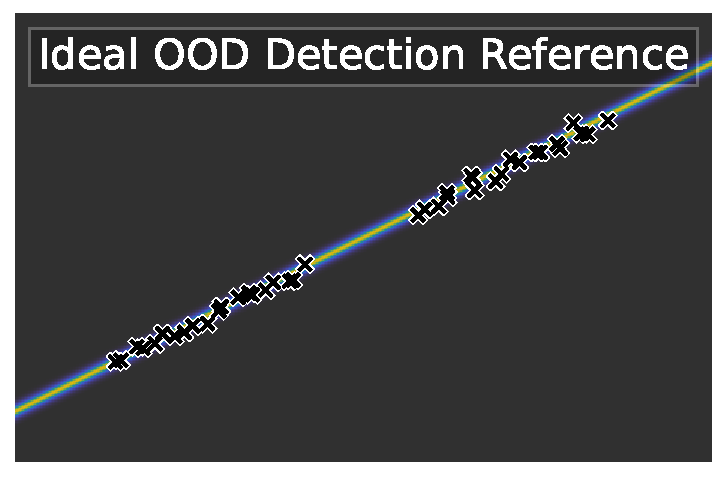
\includegraphics[width=0.388\textwidth,valign=t]{ood-detection/figures/ood-detection/confidence-line-aa-optimal.pdf}
    \end{subfigure}
    \begin{subfigure}
        \centering
        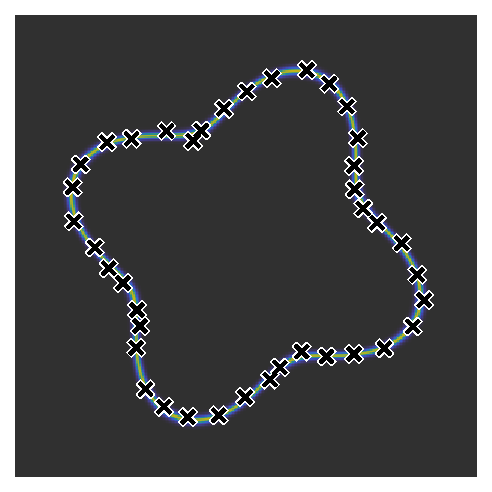
\includegraphics[width=0.254\textwidth,valign=t]{ood-detection/figures/ood-detection/confidence-circle-aa-optimal.pdf}
    \end{subfigure}
    \begin{subfigure}
        \centering
        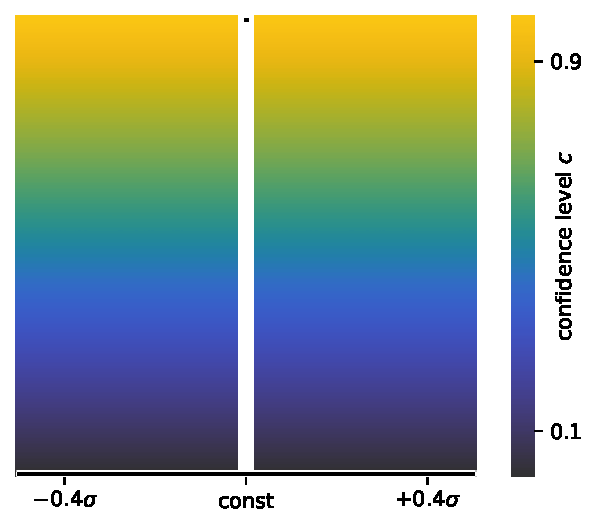
\includegraphics[width=0.308\textwidth,valign=t]{ood-detection/figures/ood-detection/confidence-haystack-aa-optimal.pdf}
    \end{subfigure}

    \vspace{-0.25em}
    \caption[Reference Example of one ideal OOD Detector]{By-example (see \Cref{txt:ood-detection-comparison}) evaluation of one possible ideal OOD detection method.}
    \label{fig:ideal-ood-detection}
\end{figure}

\noindent Let us start by comparing what these plots could look like for an ideal OOD detector with one-class SVM, an unsupervised classification method first described in \textcite{ood-svm-1999}. This method trains a support vector machine on ID inputs, assigning them a positive score, while OOD inputs get a negative score. In \Cref{fig:ideal-ood-detection}, we can see that our interpretation of an ideal OOD detector is able to succinctly extract the line and circle boundary ID subspaces in the first two figures. Note that the lines look very thin since the percentile-based confidence score from \Cref{eq:dime-id-percentile} uniformly spreads the confidence values across all ID inputs. In contrast, the washed-out two-hill confidence map in \Cref{fig:one-class-ood-detection} shows that one-class SVM only recognises that two groups of ID points are given but not that only points along that line should have high confidence. For the middle circle example, it incorrectly classifies most of the full circle as ID, even though the training data only lies on its boundary. Finally, in the haystack example, our ideal OOD detector assigns high confidence only to inputs that have the same feature value as the constant seen in training. Specifically, there is only a single black high-confidence dot on the white constant line. One-class SVM instead spreads its confidence values uniformly, meaning it is unable to identify the haystack as OOD.

\begin{figure}[H]
    \centering
    \begin{subfigure}
        \centering
        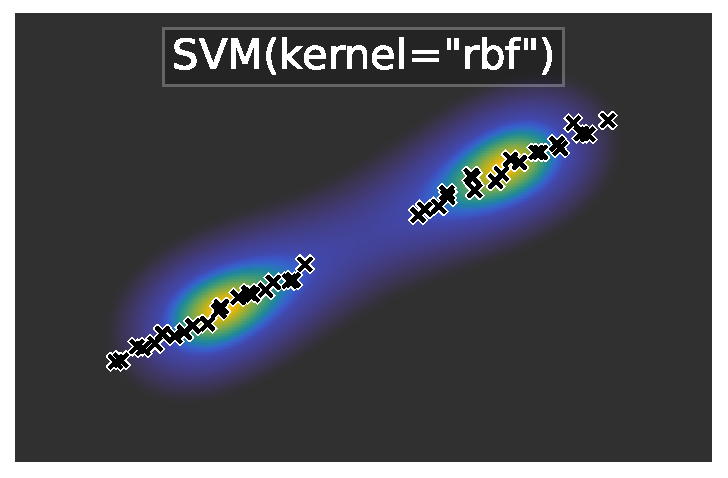
\includegraphics[width=0.388\textwidth,valign=t]{ood-detection/figures/ood-detection/confidence-line-svm-rbf.pdf}
    \end{subfigure}
    \begin{subfigure}
        \centering
        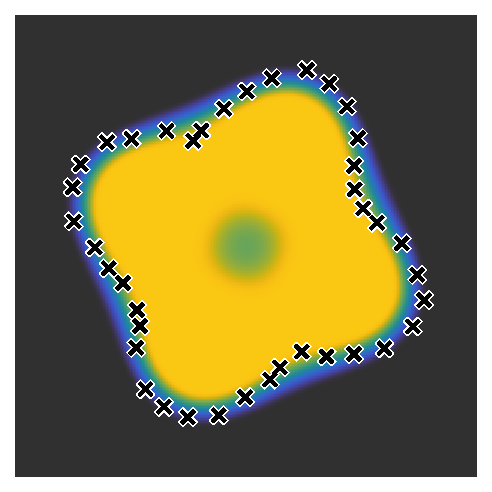
\includegraphics[width=0.254\textwidth,valign=t]{ood-detection/figures/ood-detection/confidence-circle-svm-rbf.pdf}
    \end{subfigure}
    \begin{subfigure}
        \centering
        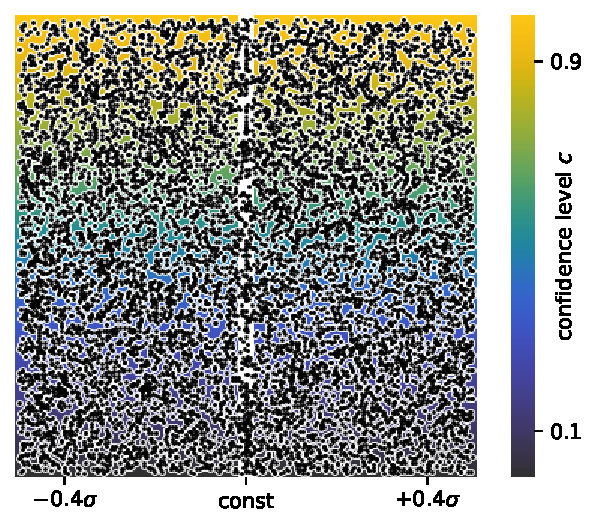
\includegraphics[width=0.308\textwidth,valign=t]{ood-detection/figures/ood-detection/confidence-haystack-svm-rbf.pdf}
    \end{subfigure}

    \caption[The One-class SVM OOD detection method]{By-example (see \Cref{txt:ood-detection-comparison}) evaluation of the One-class SVM \cite{ood-svm-1999} OOD detection method.}
    \label{fig:one-class-ood-detection}
\end{figure}

\subsection{Distance- and Isolation-based Methods}

The Mahalanobis distance (see \Cref{eq:mahalanobis-distance}) treats the ID data as a multivariate Gaussian random variable and measures how much the unseen data deviates from it. \Cref{fig:md-lof-ood-detection} shows that while this method fits the line data well (by squeezing an ellipsoid decision boundary around it), it fails for the circle and haystack test cases.

\begin{figure}[H]
    \centering
    \begin{subfigure}
        \centering
        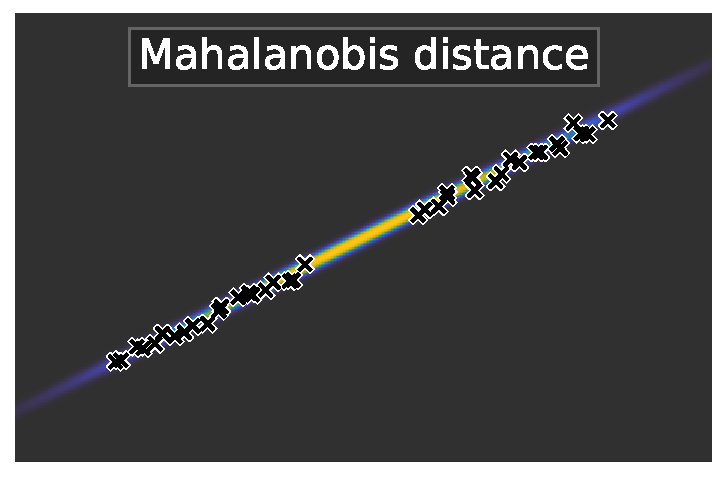
\includegraphics[width=0.388\textwidth,valign=t]{ood-detection/figures/ood-detection/confidence-line-mahalanobis.pdf}
    \end{subfigure}
    \begin{subfigure}
        \centering
        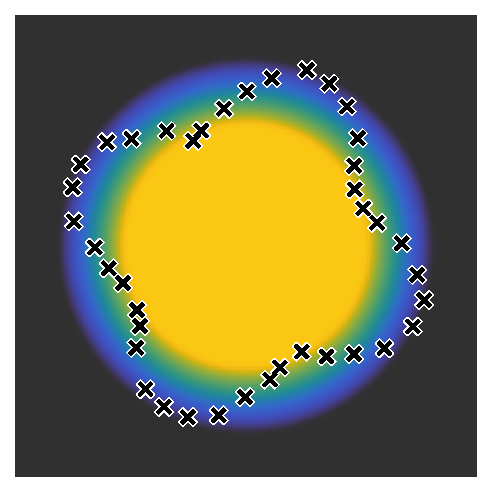
\includegraphics[width=0.254\textwidth,valign=t]{ood-detection/figures/ood-detection/confidence-circle-mahalanobis.pdf}
    \end{subfigure}
    \begin{subfigure}
        \centering
        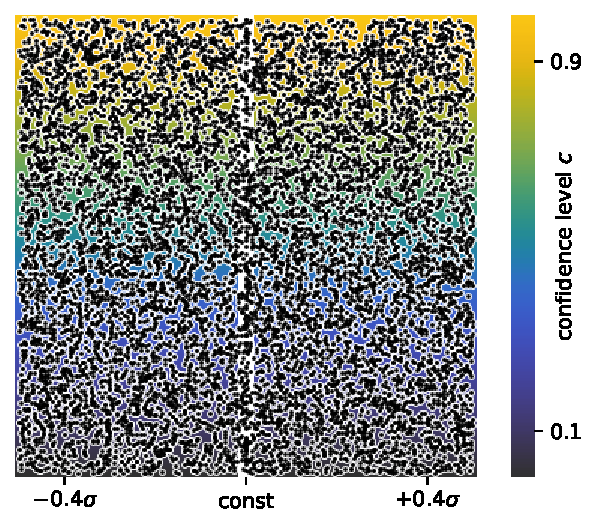
\includegraphics[width=0.308\textwidth,valign=t]{ood-detection/figures/ood-detection/confidence-haystack-mahalanobis.pdf}
    \end{subfigure}

    \begin{subfigure}
        \centering
        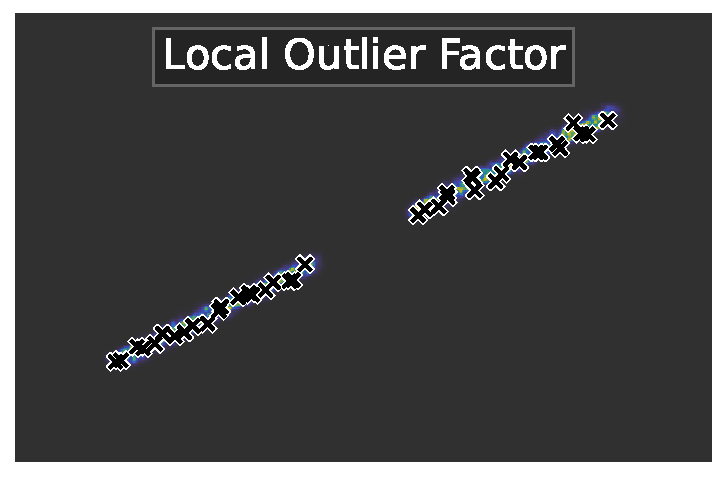
\includegraphics[width=0.388\textwidth,valign=t]{ood-detection/figures/ood-detection/confidence-line-lof.pdf}
    \end{subfigure}
    \begin{subfigure}
        \centering
        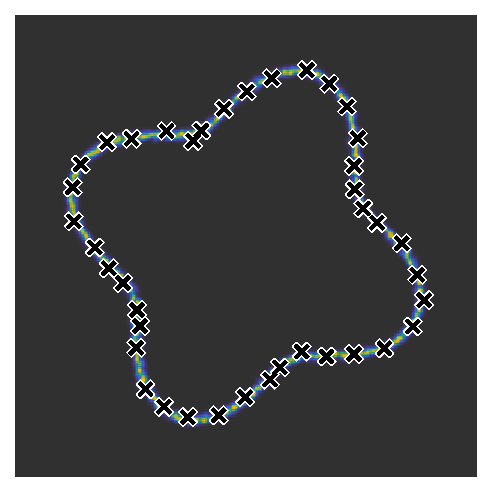
\includegraphics[width=0.254\textwidth,valign=t]{ood-detection/figures/ood-detection/confidence-circle-lof.pdf}
    \end{subfigure}
    \begin{subfigure}
        \centering
        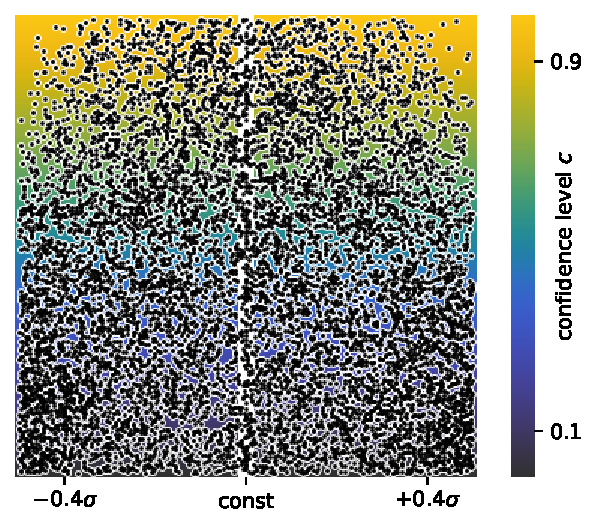
\includegraphics[width=0.308\textwidth,valign=t]{ood-detection/figures/ood-detection/confidence-haystack-lof.pdf}
    \end{subfigure}

    \caption[Distance-based OOD detection methods]{By-example (see \Cref{txt:ood-detection-comparison}) evaluation of the Mahalanobis distance (see \Cref{eq:mahalanobis-distance}) and the Local Outlier Factor (see \Cref{txt:ood-distance}) as distance-based OOD detection methods.}
    \label{fig:md-lof-ood-detection}
\end{figure}

\noindent The Local Outlier Factor (LOF, see \Cref{txt:ood-distance}) estimates the training data density around unseen data. Thus, it performs much better on the line and circle examples where the data points are closely scattered. Unlike the prior methods, the LOF classifies the gap between the two groups on the line as OOD, which may be too conservative if we assume that a machine-learning model can interpolate between the two groups. LOF is also the first method that produces slightly lower confidence for the OOD inputs in the haystack.

Isolation Forests are a non-distance-based OOD detection method by \textcite{isolation-forest-2008} and \textcite{isolation-forest-2012} that uses a forest of binary trees with random splits. OOD inputs are detected as isolated since they require fewer splits to reach a tree leaf node where they are isolated from ID inputs. Unfortunately, \Cref{fig:if-ood-detection} shows that Isolation Forests generate washed-out confidence patterns and fail for the haystack.

\begin{figure}[H]
    \centering
    \begin{subfigure}
        \centering
        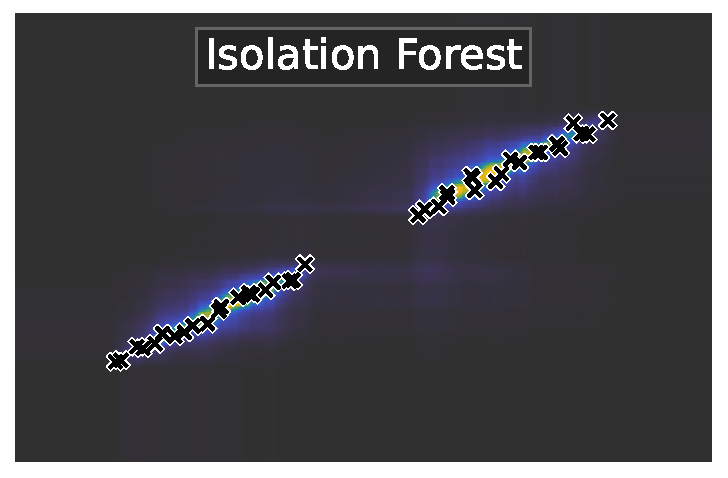
\includegraphics[width=0.388\textwidth,valign=t]{ood-detection/figures/ood-detection/confidence-line-isolation.pdf}
    \end{subfigure}
    \begin{subfigure}
        \centering
        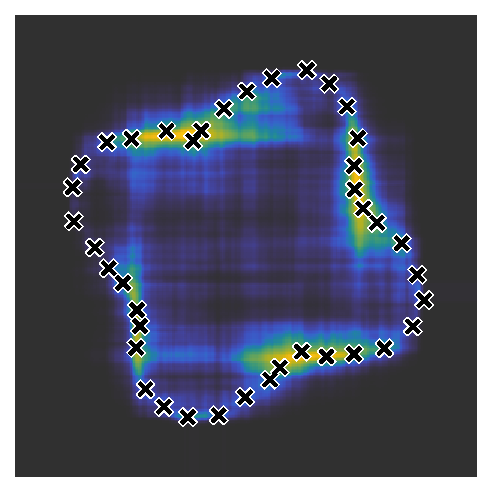
\includegraphics[width=0.254\textwidth,valign=t]{ood-detection/figures/ood-detection/confidence-circle-isolation.pdf}
    \end{subfigure}
    \begin{subfigure}
        \centering
        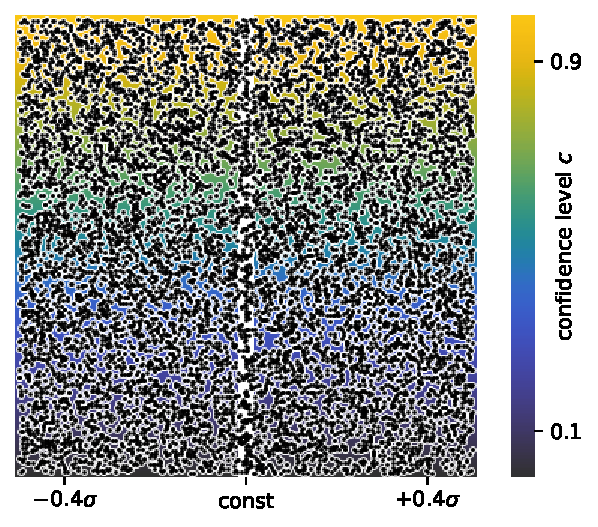
\includegraphics[width=0.308\textwidth,valign=t]{ood-detection/figures/ood-detection/confidence-haystack-isolation.pdf}
    \end{subfigure}

    \caption[Isolation Forests as an OOD detection method]{By-example (see \Cref{txt:ood-detection-comparison}) evaluation of Isolation Forests \cite{isolation-forest-2008, isolation-forest-2012} as an OOD detection method.}
    \label{fig:if-ood-detection}
\end{figure}

\subsection{Truncated PCA as a Cheap Linear Auto-Associative Method} \label{txt:truncated-pca}

In the truncated PCA method, the $d$-dimensional input data is projected onto its first $k$ principal components, where $k < d$ and chosen such that at least $95\%$ of the variance is retained. If an input can only be reconstructed from this truncated form with high error, it is OOD. \Cref{fig:truncated-pca-ood-detection} shows that the method successfully learns the line ID subspace. However, it fails in the circular example since there is no linear mapping from the 2D circle to the truncated 1st PC. In the haystack, truncated PCA displays a gradual drop in confidence for OOD inputs.

\begin{figure}[H]
    \centering
    \begin{subfigure}
        \centering
        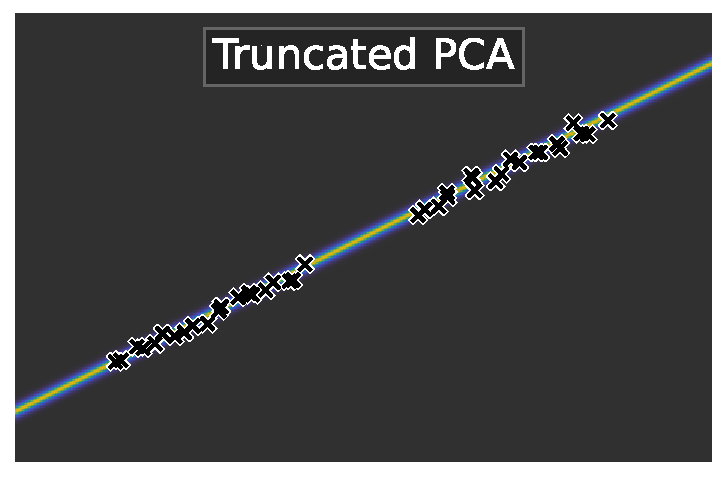
\includegraphics[width=0.388\textwidth,valign=t]{ood-detection/figures/ood-detection/confidence-line-truncated-pca.pdf}
    \end{subfigure}
    \begin{subfigure}
        \centering
        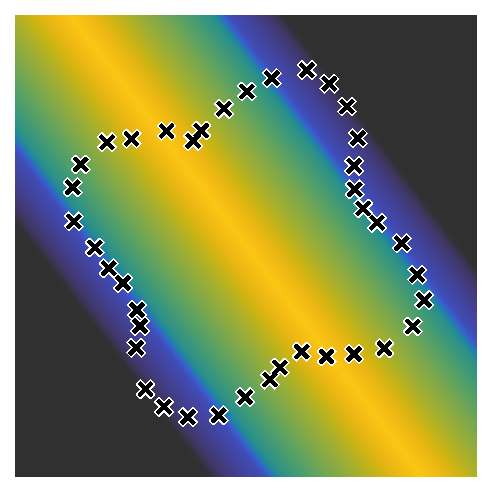
\includegraphics[width=0.254\textwidth,valign=t]{ood-detection/figures/ood-detection/confidence-circle-truncated-pca.pdf}
    \end{subfigure}
    \begin{subfigure}
        \centering
        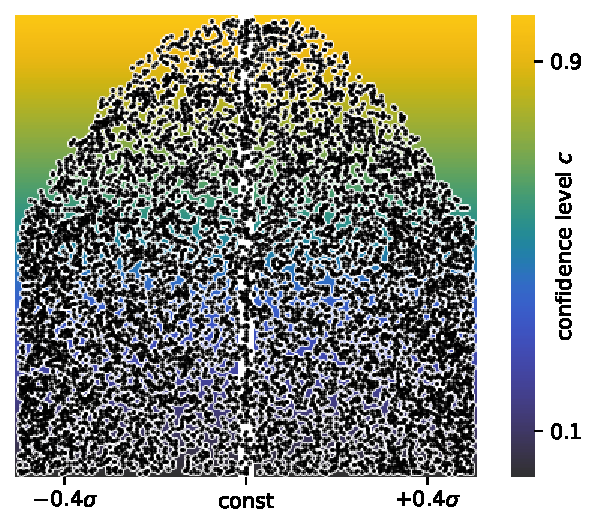
\includegraphics[width=0.308\textwidth,valign=t]{ood-detection/figures/ood-detection/confidence-haystack-truncated-pca.pdf}
    \end{subfigure}

    \caption[Truncated PCA as an OOD detection method]{By-example (see \Cref{txt:ood-detection-comparison}) evaluation of truncated PCA as an OOD detection method.}
    \label{fig:truncated-pca-ood-detection}
\end{figure}

\subsection{Exploration of diverse Auto-Associative Methods} \label{txt:ood-detection-analyis-auto-associative}

Auto-Associative Networks (see \Cref{txt:auto-associative}) are non-linear neural networks that compress and reconstruct their input. High reconstruction errors can be used as an indicator for OOD inputs. \Cref{fig:auto-associative-ood-detection} shows how auto-associative networks using the ReLU (popular) and sigmoid (recommended by \textcite{auto-associative-2001}) activation functions perform when the encoding and decoding layers have 16 neurons, and the bottleneck has one or eight for the 2D and haystack examples, respectively. While the ReLU function performs well for the haystack, it produces harsh artefacts for the circle. The sigmoid function also fails here with a solid bean shape but works for the line. As suggested by \textcite{dime-detector-2021}, we also try applying the Mahalanobis distance to the per-feature reconstruction errors instead of summing them. As shown in \Cref{fig:auto-associative-mahalanobis-ood-detection}, this produces much tighter OOD detection bounds that benefit the sigmoid activation and the haystack example, in particular.

\begin{figure}[H]
    \centering
    \begin{subfigure}
        \centering
        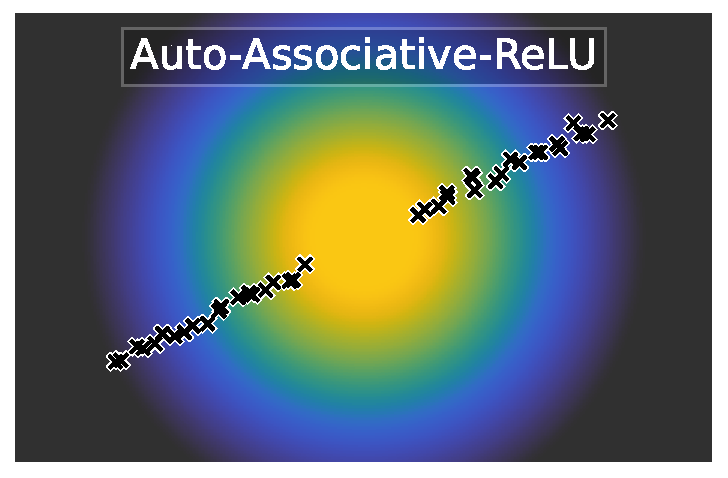
\includegraphics[width=0.388\textwidth,valign=t]{ood-detection/figures/ood-detection/confidence-line-aa-relu.pdf}
    \end{subfigure}
    \begin{subfigure}
        \centering
        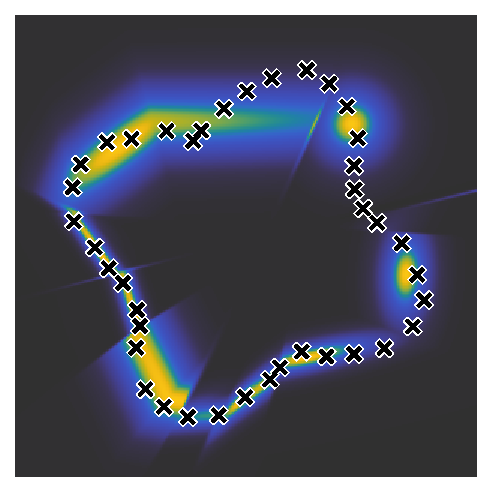
\includegraphics[width=0.254\textwidth,valign=t]{ood-detection/figures/ood-detection/confidence-circle-aa-relu.pdf}
    \end{subfigure}
    \begin{subfigure}
        \centering
        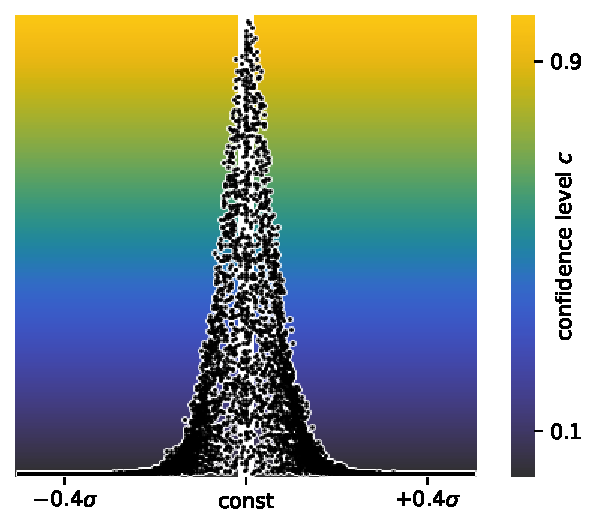
\includegraphics[width=0.308\textwidth,valign=t]{ood-detection/figures/ood-detection/confidence-haystack-aa-relu.pdf}
    \end{subfigure}

    \begin{subfigure}
        \centering
        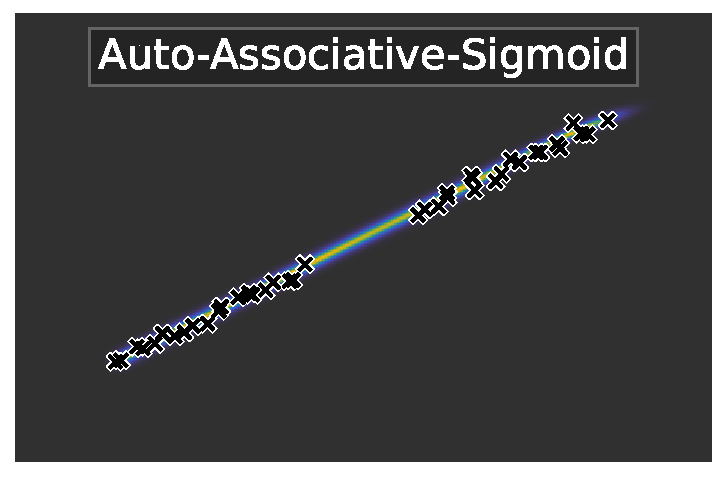
\includegraphics[width=0.388\textwidth,valign=t]{ood-detection/figures/ood-detection/confidence-line-aa-sigmoid.pdf}
    \end{subfigure}
    \begin{subfigure}
        \centering
        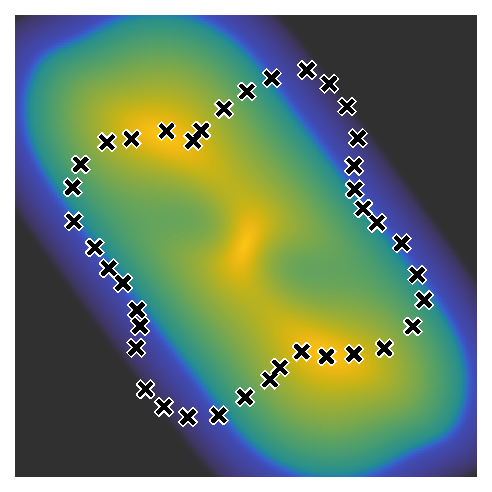
\includegraphics[width=0.254\textwidth,valign=t]{ood-detection/figures/ood-detection/confidence-circle-aa-sigmoid.pdf}
    \end{subfigure}
    \begin{subfigure}
        \centering
        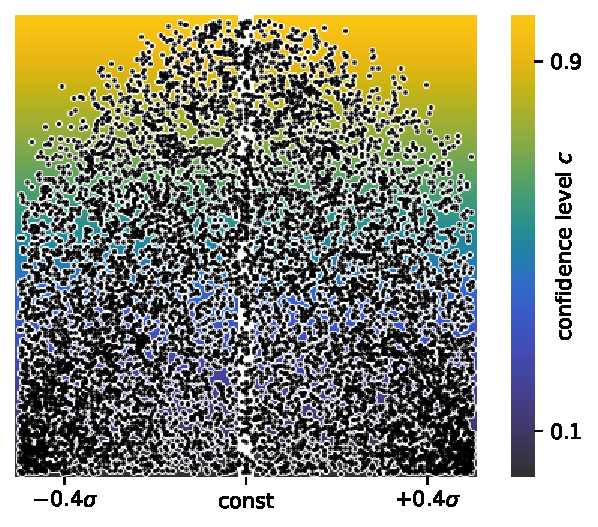
\includegraphics[width=0.308\textwidth,valign=t]{ood-detection/figures/ood-detection/confidence-haystack-aa-sigmoid.pdf}
    \end{subfigure}

    \caption[Comparison of Auto-Associative Networks as OOD detection methods]{By-example (see \Cref{txt:ood-detection-comparison}) evaluation of Auto-Associative networks (see \Cref{txt:auto-associative}) as OOD detection methods. The networks are trained with the ReLU or sigmoid activation function, and their per-feature squared reconstruction errors are summed before being transformed into a confidence score.}
    \label{fig:auto-associative-ood-detection}
\end{figure}

\begin{figure}[H]
    \centering
    \begin{subfigure}
        \centering
        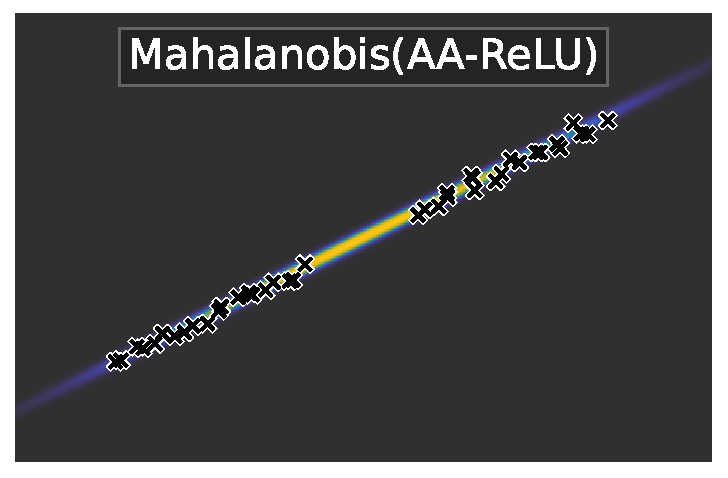
\includegraphics[width=0.388\textwidth,valign=t]{ood-detection/figures/ood-detection/confidence-line-aa-relu-mahalanobis.pdf}
    \end{subfigure}
    \begin{subfigure}
        \centering
        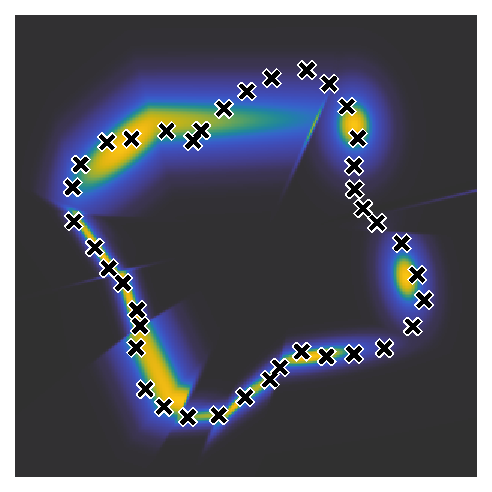
\includegraphics[width=0.254\textwidth,valign=t]{ood-detection/figures/ood-detection/confidence-circle-aa-relu-mahalanobis.pdf}
    \end{subfigure}
    \begin{subfigure}
        \centering
        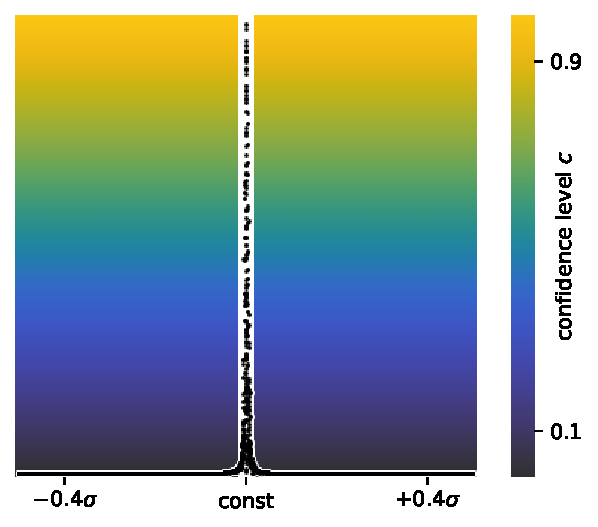
\includegraphics[width=0.308\textwidth,valign=t]{ood-detection/figures/ood-detection/confidence-haystack-aa-relu-mahalanobis.pdf}
    \end{subfigure}

    \begin{subfigure}
        \centering
        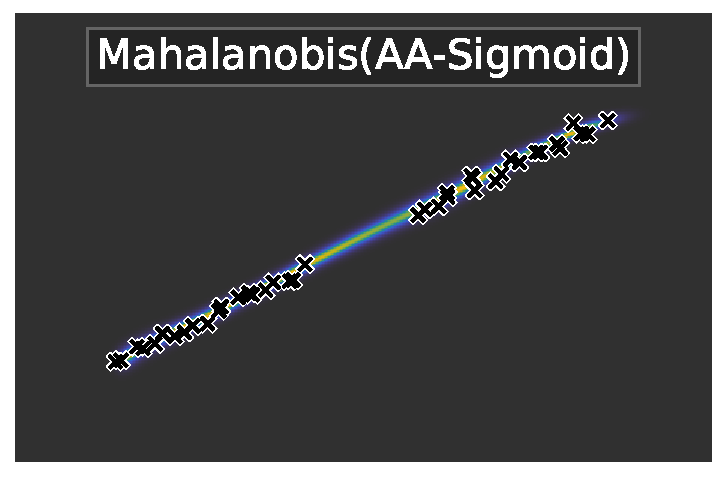
\includegraphics[width=0.388\textwidth,valign=t]{ood-detection/figures/ood-detection/confidence-line-aa-sigmoid-mahalanobis.pdf}
    \end{subfigure}
    \begin{subfigure}
        \centering
        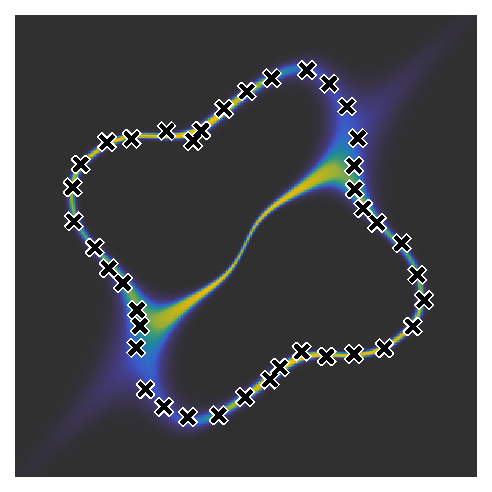
\includegraphics[width=0.254\textwidth,valign=t]{ood-detection/figures/ood-detection/confidence-circle-aa-sigmoid-mahalanobis.pdf}
    \end{subfigure}
    \begin{subfigure}
        \centering
        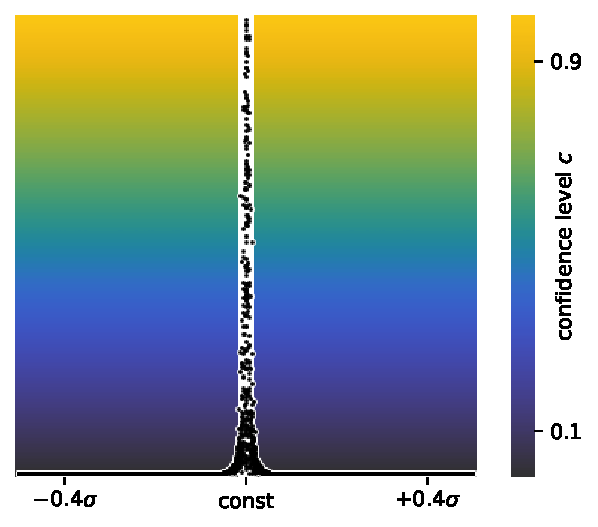
\includegraphics[width=0.308\textwidth,valign=t]{ood-detection/figures/ood-detection/confidence-haystack-aa-sigmoid-mahalanobis.pdf}
    \end{subfigure}

    \caption[Comparison of Mahalanobis-transformed Auto-Associative Networks as OOD detection methods]{By-example (see \Cref{txt:ood-detection-comparison}) evaluation of Auto-Associative networks (see \Cref{txt:auto-associative}) as OOD detection methods. The networks use the ReLU or sigmoid activation function, and their per-feature reconstruction errors are transformed into a confidence score via the Mahalanobis distance (see \Cref{eq:mahalanobis-distance}).}
    \label{fig:auto-associative-mahalanobis-ood-detection}
\end{figure}

\noindent The bad fits generated by the ReLU activation function for the line example and the sigmoid activation function for the circular case motivate the exploration of Gaussian Processes (GPs, see \Cref{txt:gaussian-process}) as an auto-associative predictor. While using GPs as an uncertainty-based method for OOD detection is discussed in \Cref{txt:ood-detection-analysis-uq}, here they are fit on the input $X$ to predict $X$ such that the auto-associative prediction uncertainty and error can be measured. \Cref{fig:auto-associative-gp-ood-detection} highlights two possible approaches.

\begin{figure}[H]
    \centering
    \begin{subfigure}
        \centering
        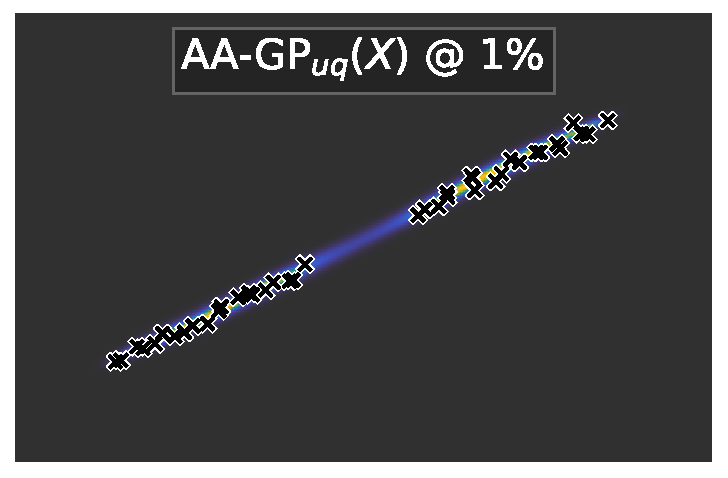
\includegraphics[width=0.388\textwidth,valign=t]{ood-detection/figures/ood-detection/confidence-line-gp-coarse-xx.pdf}
    \end{subfigure}
    \begin{subfigure}
        \centering
        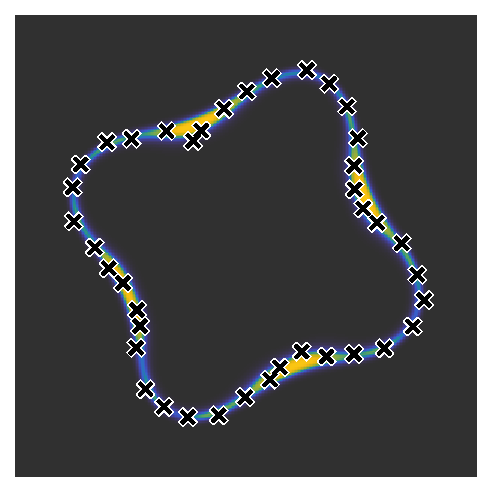
\includegraphics[width=0.254\textwidth,valign=t]{ood-detection/figures/ood-detection/confidence-circle-gp-coarse-xx.pdf}
    \end{subfigure}
    \begin{subfigure}
        \centering
        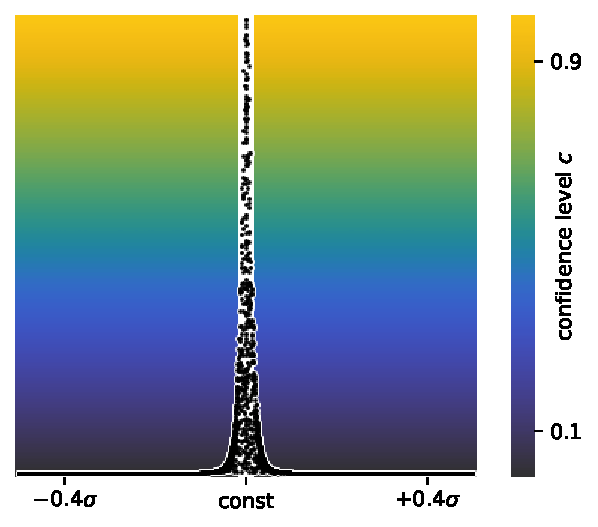
\includegraphics[width=0.308\textwidth,valign=t]{ood-detection/figures/ood-detection/confidence-haystack-gp-coarse-xx.pdf}
    \end{subfigure}

    \begin{subfigure}
        \centering
        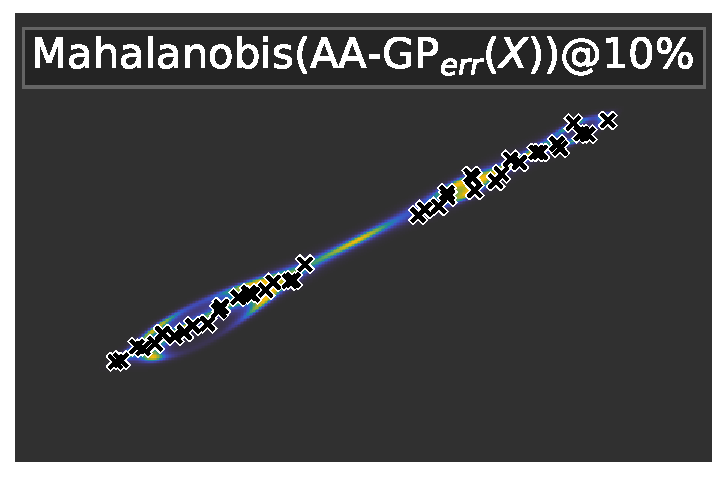
\includegraphics[width=0.388\textwidth,valign=t]{ood-detection/figures/ood-detection/confidence-line-gp-xx-mahalanobis.pdf}
    \end{subfigure}
    \begin{subfigure}
        \centering
        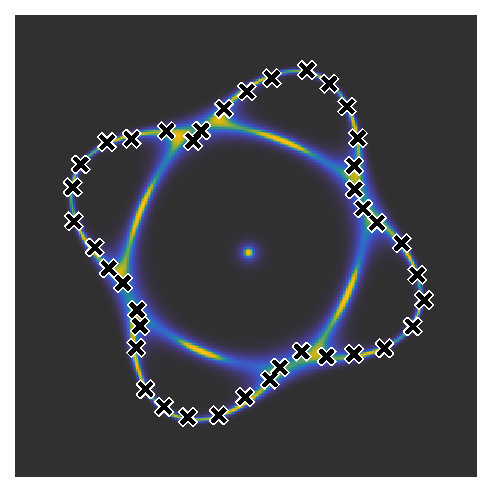
\includegraphics[width=0.254\textwidth,valign=t]{ood-detection/figures/ood-detection/confidence-circle-gp-xx-mahalanobis.pdf}
    \end{subfigure}
    \begin{subfigure}
        \centering
        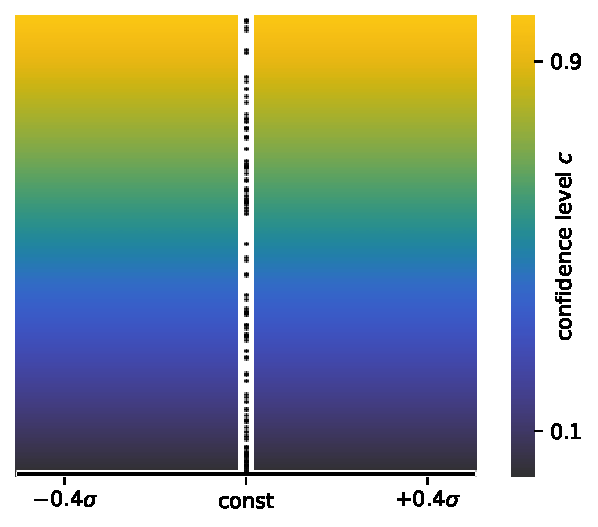
\includegraphics[width=0.308\textwidth,valign=t]{ood-detection/figures/ood-detection/confidence-haystack-gp-xx-mahalanobis.pdf}
    \end{subfigure}

    \caption[Comparison of Auto-Associative Gaussian Processes as OOD detection methods]{By-example (see \Cref{txt:ood-detection-comparison}) evaluation of Auto-Associative (see \Cref{txt:auto-associative}) Gaussian Processes (see \Cref{txt:gaussian-process}), optionally using the Mahalanobis distance (see \Cref{eq:mahalanobis-distance}), as OOD detection methods.}
    \label{fig:auto-associative-gp-ood-detection}
\end{figure}

\noindent In the first approach, the auto-associative GP predicts per-feature-uncertainties, which are summed up and transformed into an OOD confidence score. This method works remarkably well on all three examples, even when trained on just $1\%$ of the available training data. In the line example, a 1D ID-input subspace may be preferable, such as the one the truncated PCA method extracts in \Cref{fig:truncated-pca-ood-detection}. However, producing high confidence around the training points and allowing some lower-confidence interpolation in between also provides valuable OOD detection. Furthermore, this method generates similarly tight confidence spikes as the auto-associative networks using the Mahalanobis distance.

The second approach compares the auto-associative GP's mean predictions with the original input. The per-feature errors, which are summed or transformed with the Mahalanobis distance, produce the confidence score. Unfortunately, while this method generates an even thinner spike in the haystack example, it also produces artefacts in the line and circle examples, both with and without the Mahalanobis distance.

\subsection{Surprisingly Successful Uncertainty-based Methods} \label{txt:ood-detection-analysis-uq}

\begin{figure}[H]
    \centering
    \begin{subfigure}
        \centering
        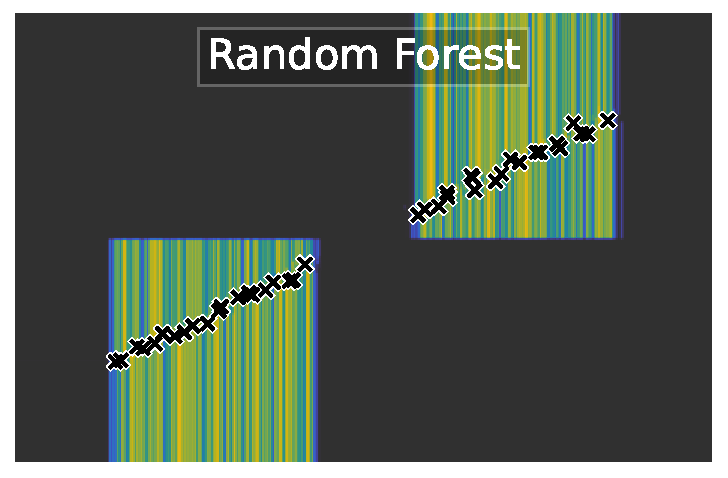
\includegraphics[width=0.388\textwidth,valign=t]{ood-detection/figures/ood-detection/confidence-line-rf.pdf}
    \end{subfigure}
    \begin{subfigure}
        \centering
        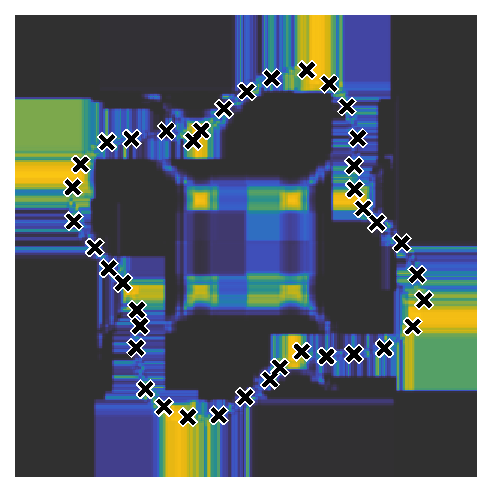
\includegraphics[width=0.254\textwidth,valign=t]{ood-detection/figures/ood-detection/confidence-circle-rf.pdf}
    \end{subfigure}
    \begin{subfigure}
        \centering
        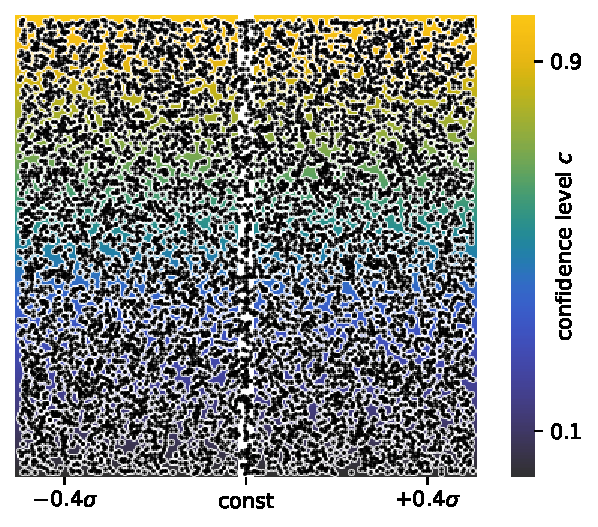
\includegraphics[width=0.308\textwidth,valign=t]{ood-detection/figures/ood-detection/confidence-haystack-rf.pdf}
    \end{subfigure}

    \caption[Random Forest Uncertainty for OOD Detection]{By-example (see \Cref{txt:ood-detection-comparison}) evaluation of using Random Forest (see \Cref{txt:ensembles-decision-tree-random-forest}) ensemble prediction variation for OOD detection.}
    \label{fig:uq-rf-ood-detection}
\end{figure}

Model uncertainty and confidence are not equivalent. While the former describes the expected prediction error, the latter determines whether a prediction of the target value and its uncertainty can be used at all. Therefore, OOD uncertainty estimates are only valuable if the model is constructed and trained to have high uncertainty on inputs that deviate from the ID training data. If this is the case, it can be convenient to use unexpectedly high prediction uncertainty as a proxy for low confidence. In this subsection, we evaluate two uncertainty-based methods for OOD detection. In each, a model is trained on the ID input-output pairs, and its prediction uncertainty on unseen data is translated into a confidence score.

Random Forests (RFs) (see \Cref{txt:ensembles-decision-tree-random-forest}) are a generalist method that utilises bootstrapping to produce high-quality predictions even in higher dimensions and without hyperparameter-tuning \cite{ml-hyperparameters-2021}. However, RFs are also prone to overgeneralising where possible. For example, \Cref{fig:uq-rf-ood-detection} shows that the high-confidence areas extracted by analysing the variance across the forest's predictions have outgoing streaks that reach infinitely far into the OOD space. RFs also fail to find any difference between ID and OOD inputs in the haystack task.

\begin{figure}[H]
    \centering
    \begin{subfigure}
        \centering
        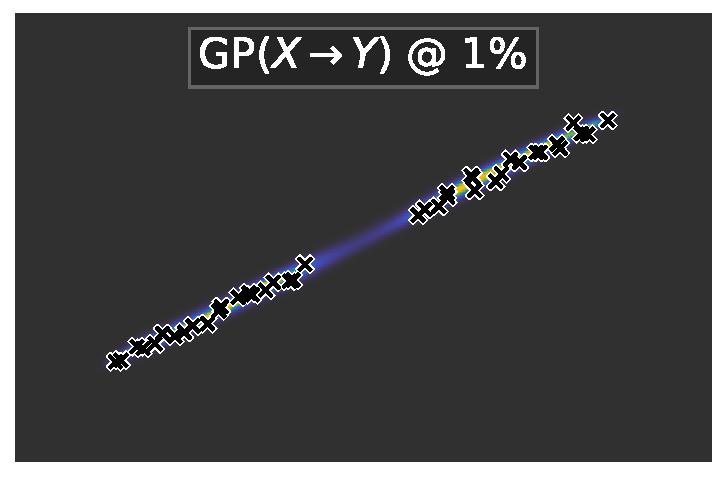
\includegraphics[width=0.388\textwidth,valign=t]{ood-detection/figures/ood-detection/confidence-line-gp-coarse-xy.pdf}
    \end{subfigure}
    \begin{subfigure}
        \centering
        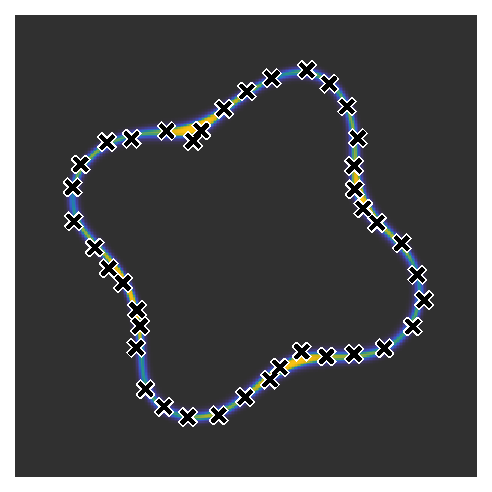
\includegraphics[width=0.254\textwidth,valign=t]{ood-detection/figures/ood-detection/confidence-circle-gp-coarse-xy.pdf}
    \end{subfigure}
    \begin{subfigure}
        \centering
        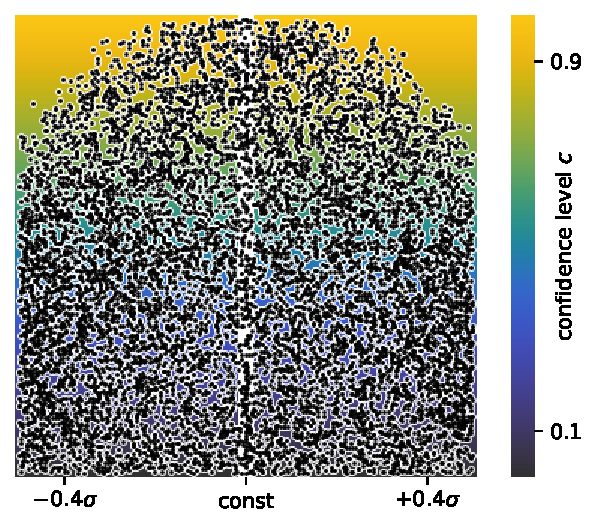
\includegraphics[width=0.308\textwidth,valign=t]{ood-detection/figures/ood-detection/confidence-haystack-gp-coarse-xy.pdf}
    \end{subfigure}

    \begin{subfigure}
        \centering
        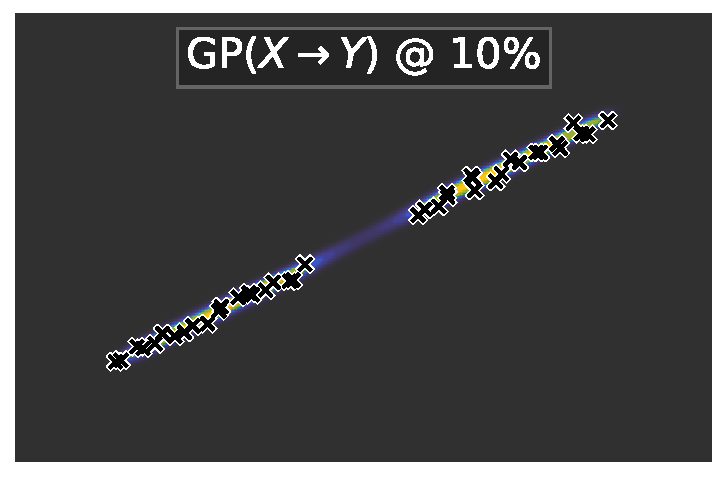
\includegraphics[width=0.388\textwidth,valign=t]{ood-detection/figures/ood-detection/confidence-line-gp.pdf}
    \end{subfigure}
    \begin{subfigure}
        \centering
        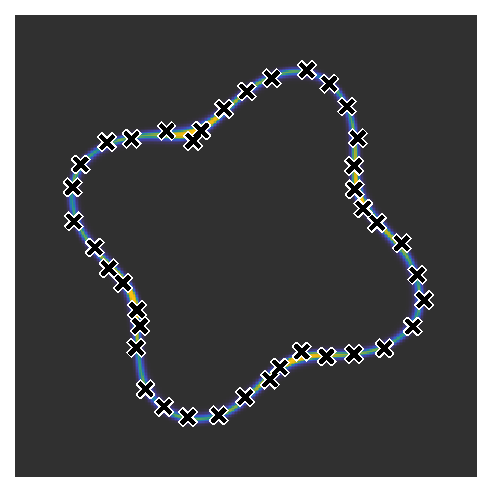
\includegraphics[width=0.254\textwidth,valign=t]{ood-detection/figures/ood-detection/confidence-circle-gp.pdf}
    \end{subfigure}
    \begin{subfigure}
        \centering
        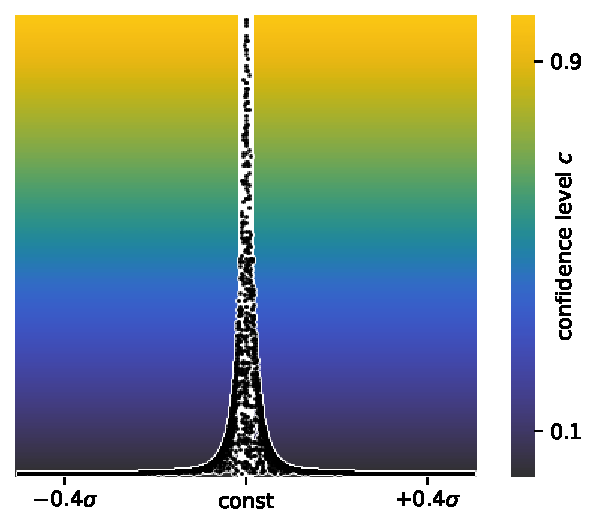
\includegraphics[width=0.308\textwidth,valign=t]{ood-detection/figures/ood-detection/confidence-haystack-gp.pdf}
    \end{subfigure}

    \caption[Gaussian Process uncertainty for OOD detection]{By-example (see \Cref{txt:ood-detection-comparison}) evaluation of Gaussian Processes (see \Cref{txt:gaussian-process}) with different training data subsample sizes as OOD detection methods.}
    \label{fig:uq-gp-ood-detection}
\end{figure}

\noindent Gaussian Processes (see \Cref{txt:gaussian-process}) are a stochastic method to smoothly fit a function to a given set of training points \cite{gp-ml-2005}. Given their high computational complexity, $\text{O}(N^3)$ for $N$ data points, fitting them is expensive and often only possible using approximation or a subset of the data. \Cref{fig:uq-gp-ood-detection} shows that while a GP trained on just $1\%$ of the data already performs very well in the line and circle cases, it only produces a very gradual drop in confidence for the haystack. At $10\%$ of the data and 1000-times the computational cost, the GP shows a much better confidence peak similar to the ones produced by auto-associative methods in \Cref{txt:ood-detection-analyis-auto-associative}.

\subsection{Challenges with Noise-Contrastive Priors} \label{txt:ood-detection-analysis-ncp}

\Cref{txt:uq-conf-method} summarises how \textcite{noise-contrastive-uq-2020} use noise-contrastive priors to train a probabilistic model to have high uncertainty for OOD inputs. Inspired by their work, we also test whether training the uncertainty-based OOD detectors with probably-OOD perturbed input-output pairs alongside the ID points improves their OOD detection. \Cref{fig:ncp-gp-rf-ood-detection} shows that their effectiveness varies.

For Gaussian Processes, they smudge the high-confidence areas to span more OOD inputs since they now contain \textit{some} training samples. While no effect on the circular example can be observed, the noise-contrastive GPs fail entirely for the haystack, even though standard GPs handle that case well. This failure highlights that inventing OOD inputs for training may confuse sensitive models such as Gaussian processes. \Cref{txt:ood-synthesis-analysis} explores different strategies for training with synthetic OOD samples.

For Random Forests, however, the noise-contrastive method provides a clear improvement. Training them with high-uncertainty noise-perturbed inputs alongside the OOD data forces the RFs to learn a tight boundary around the ID inputs, removing the over-generalising high-confidence streaks seen in \Cref{fig:uq-rf-ood-detection}, and thus bringing their performance almost on par with the Local Outlier Factor (see \Cref{fig:md-lof-ood-detection}). Note, however, that the confidence maps produced by the RF also contain widespread subtle noise artefacts, and that the RF still fails to succinctly identify OOD inputs in the haystack example.

\begin{figure}[H]
    \centering
    \begin{subfigure}
        \centering
        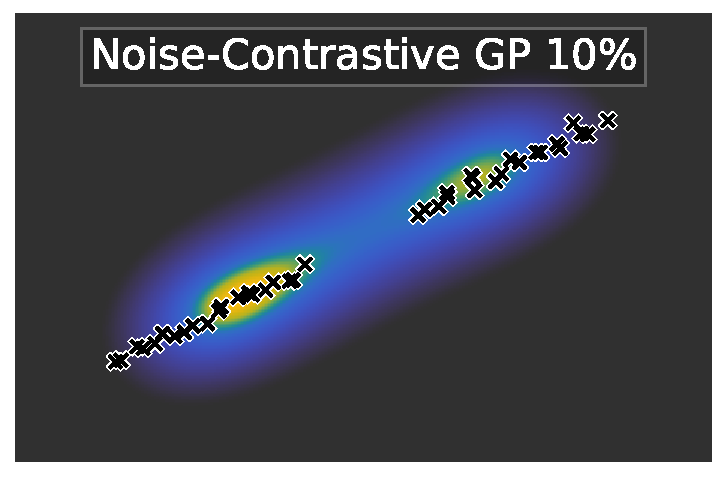
\includegraphics[width=0.388\textwidth,valign=t]{ood-detection/figures/ood-detection/confidence-line-nc-gp.pdf}
    \end{subfigure}
    \begin{subfigure}
        \centering
        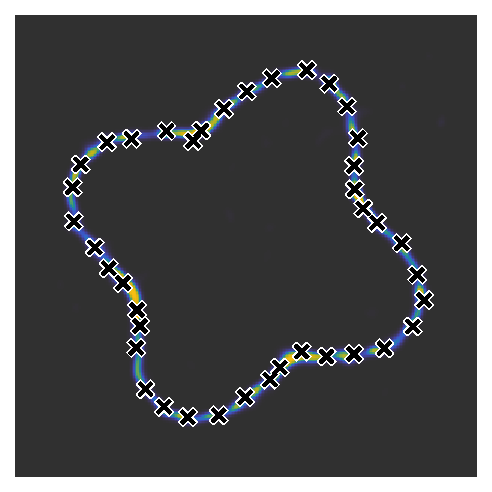
\includegraphics[width=0.254\textwidth,valign=t]{ood-detection/figures/ood-detection/confidence-circle-nc-gp.pdf}
    \end{subfigure}
    \begin{subfigure}
        \centering
        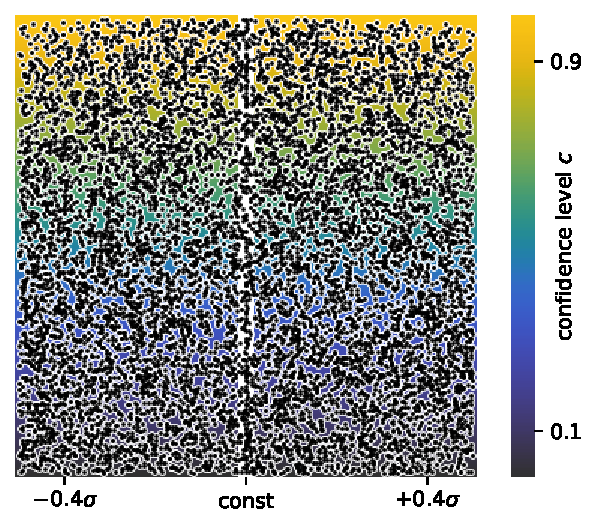
\includegraphics[width=0.308\textwidth,valign=t]{ood-detection/figures/ood-detection/confidence-haystack-nc-gp.pdf}
    \end{subfigure}

    \begin{subfigure}
        \centering
        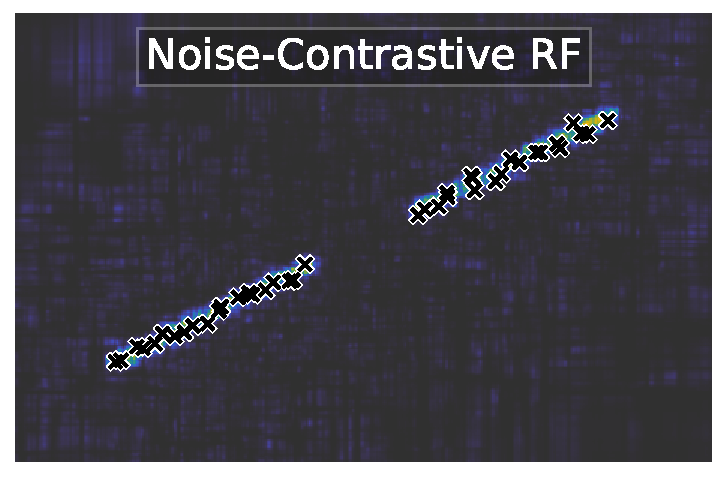
\includegraphics[width=0.388\textwidth,valign=t]{ood-detection/figures/ood-detection/confidence-line-nc-rf.pdf}
    \end{subfigure}
    \begin{subfigure}
        \centering
        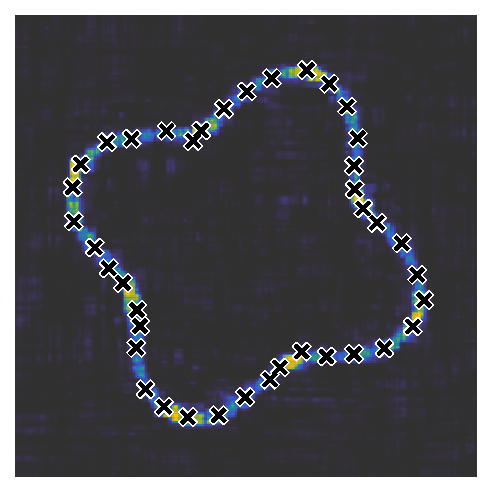
\includegraphics[width=0.254\textwidth,valign=t]{ood-detection/figures/ood-detection/confidence-circle-nc-rf.pdf}
    \end{subfigure}
    \begin{subfigure}
        \centering
        \includegraphics[width=0.308\textwidth,valign=t]{ood-detection/figures/ood-detection/confidence-haystack-nc-rf.pdf}
    \end{subfigure}

    \caption[Noise-Contrastive Priors for OOD detection]{By-example (see \Cref{txt:ood-detection-comparison}) evaluation of Noise-Contrastive Priors (see \Cref{txt:uq-conf-method}) for Gaussian Processes (see \Cref{txt:gaussian-process}) and Random Forests (see \Cref{txt:ensembles-decision-tree-random-forest}) as OOD detection methods.}
    \label{fig:ncp-gp-rf-ood-detection}
\end{figure}

\subsection{Recommendations for OOD Detection Methods} \label{txt:ood-detection-summary}

This section has visually evaluated several OOD detection methods based on three simple and intuitive test cases. We have developed these three toy examples to catch potential OOD detection failure cases early -- if a method does not work in these 2D examples, how can we trust it to work on high-dimensional data where it is much more challenging to define what non-trivial OOD inputs look like?

\newpar From these experiments, we can provide the following recommendations:
\begin{enumerate}
    \item If the dimensionality is low, ID samples are uniformly spread within the ID subspace, and conceptual generalisation to unseen data is not as important, the Local Outlier Factor provides a very simple yet effective method.
    \item If conceptual generalisation is desired, auto-associative networks provide an intuitive method for identifying the ID subspace. However, these neural networks require additional tuning to reduce the confidence map artefacts generated from suboptimal training. Applying the Mahalanobis distance to the reconstruction errors generally improves the confidence map quality. If the ID subspace is linear, truncated PCA provides a cheaper implementation than neural networks.
    \item Gaussian Process uncertainty performs surprisingly well across all examples at detecting OOD. However, their computational cost and decreased performance in higher dimensions limit their applicability.
\end{enumerate}

\noindent In this work, we focus on fitting a response surface model for the SOSAA simulation. Thus, conceptual generalisation is desirable, and we choose to explore auto-associative networks for OOD detection further.

\section{Toy-Comparisons of OOD Synthesis Methods} \label{txt:ood-synthesis-analysis}

\Cref{txt:ood-detection-comparison} has analysed the performance of different OOD detection methods using three toy examples. Most of these methods, excluding noise-contrastive priors, only use ID inputs to train their detectors since often no OOD samples are available. However, tasks such as providing meaningful OOD confidence scores, which \Cref{txt:confidence-scoring-comparison} explores, benefit from being trained with both ID and OOD samples \cite{ood-exposure-2018}. Specifically, examples of OOD inputs provide tangible signals during training as to where to strike the balance between which inputs should be accepted as ID with high confidence and for which the model should be weary. Having OOD samples thus makes it easier to integrate OOD detection with other tasks in a joint model loss function.

However, training with OOD samples requires actually having access to OOD samples. While OOD datasets exist for some tasks, such as image recognition, synthesising OOD inputs is a more flexible and powerful approach. \Cref{txt:ood-input-generation} provides an overview of the Boundary Aware Learning method \cite{ood-boundary-2021}, which serves as inspiration for the techniques explored in this section.

\newpar As in the previous section, the comparison figures are split into three columns that highlight each method's performance across three toy examples: (1)st two groups of points on a line, (2)nd points on the boundary of a sine-perturbed circle, and (3)rd a 10-dimensional multivariate normal distribution in which one feature is constant. Please refer to \Cref{txt:ood-detection-comparison} for a more detailed introduction to these toy examples. Given the ID input points for each toy example, each method is tasked with generating synthetic OOD inputs. Next, a multi-layer classifier is trained on both the ID and synthetic OOD inputs using the default settings in the \texttt{scikit-learn} library \cite{scikit-learn-2011}. Specifically, the network has one layer with 100 neurons using the ReLU activation function, which provides a level playing ground for all tested methods. This classifier's predicted probability that an input is in-distribution is then used as the ID confidence value. Each plot shows the predicted confidence for points surrounding the ID inputs using the CET-L20 colour map \cite{color-cet-2015, color-cet-2023} from black for OOD over blue and green to yellow for ID points. A subsample of the ID inputs is shown as black \texttt{x} markers, and some of the synthetic OOD inputs are shown as white dots. The haystack example plots are again adapted for their high dimensionality and only show the distribution of ID confidence values on the y-axis for different inputs for the constant feature on the x-axis. The location of the constant seen in training is highlighted as a white line. Since the confidence detection model is the same across all methods, these figures only evaluate the effect that the OOD synthesis has on the performance of the detector. Ideally, the detector should be highly confident in ID inputs, classify most of the input feature space as OOD, and produce a tight and sharp boundary around the ID manifold.

\subsection{Trivial Random OOD Inputs as a Baseline} \label{txt:uniform-ood-synthesis-analysis}

The most trivial technique for generating synthetic OOD inputs is to sample random noise, which is used in many methods \cite[e.g.][]{ood-class-2022, ood-boundary-2021, ood-training-2017, ood-exposure-confidence-2021, learning-ood-confidence-2018, noise-contrastive-uq-2020}. While normal-distributed samples, drawn independently per feature, may provide the desired coverage of the input space for some input domains, we follow \textcite{ood-boundary-2021} and use uniformly distributed random inputs but widen their range slightly beyond the training data. While we could also generate random output labels and train a detector on the increased uncertainty for OOD inputs as \textcite{noise-contrastive-uq-2020} propose, \Cref{txt:uq-conf-method} and \Cref{txt:ood-detection-analysis-ncp} have already explored this approach and its flaws. To avoid having to assume a fixed output range, we only generate synthetic OOD inputs.

\begin{figure}[H]
    \centering
    \begin{subfigure}
        \centering
        \includegraphics[width=0.388\textwidth,valign=t]{ood-detection/figures/ood-synthesis/ood-line-uniform.pdf}
    \end{subfigure}
    \begin{subfigure}
        \centering
        \includegraphics[width=0.254\textwidth,valign=t]{ood-detection/figures/ood-synthesis/ood-circle-uniform.pdf}
    \end{subfigure}
    \begin{subfigure}
        \centering
        \includegraphics[width=0.308\textwidth,valign=t]{ood-detection/figures/ood-synthesis/ood-haystack-uniform.pdf}
    \end{subfigure}

    \caption[Random Synthetic OOD Samples]{By-example (see \Cref{txt:ood-synthesis-analysis}) evaluation of uniformly sampling OOD inputs.}
    \label{fig:uniform-ood-samples}
\end{figure}

\noindent \Cref{fig:uniform-ood-samples} shows that just by sampling OOD inputs uniformly, the OOD detector already learns reasonable boundaries for the line and circle examples. Note that in the line example, the extracted ID subspace is cut off since no ID samples are present in the lower left corner, and the ReLU activation function used in the neural network OOD detector is prone to cutting off some of the input space if possible. In the circle toy example, this simple method produces a box-like outline that roughly fits the circle boundary. Note, however, that the detector is never fully confident, even very close to the ID inputs, since many uniformly sampled OOD inputs overlap with the ID space. Unfortunately, uniformly sampling OOD inputs fails entirely on the haystack example as the OOD detector is unable to identify any OOD inputs and instead classifies all inputs as ID.

\subsection{Adversarial OOD Inputs using the Fast Gradient Sign Method} \label{txt:adversarial-ood-synthesis-analysis}

Adversarial methods provide a more targeted approach to generating OOD inputs. In the following experiments, we test the cheap Fast Gradient Sign Method (FGSM) \cite{fast-gradient-2014}. Given some input $x$ and a predictor $f(x)$, it finds a small perturbation that significantly increases the prediction error $E(x)$:
\begin{equation*}
    x' = x + \epsilon \cdot \text{sign} \left( \frac{\partial E(x)}{\partial x} \right)
\end{equation*}
where $\epsilon$ is the perturbation step length and $E(x)$ is some prediction error function. Given the success of auto-associative networks in learning the ID input subspace in \Cref{txt:ood-detection-analyis-auto-associative}, we reuse them here to provide reconstruction error gradients. For these experiments, we manually implement a `perfect' auto-associative mapping. Thus, only the FGSM method, but not its source of gradients, is evaluated. For instance, the perfect auto-associative mappings for the line and circle toy examples reconstruct an input point by projecting it onto the exact line and circle boundary from which the ID points were sampled with noise. In the haystack example, the reconstruction simply resets the constant-in-training feature to the constant value seen during training. It is also worth noting that the FGSM method is not directly applied to the ID training points but to a random sample of points generated from a Gaussian kernel density estimation of the ID training data (see \Cref{txt:online-distribution-fitting}).

The first row in \Cref{fig:fgsm-t-poking-ood-samples} shows that the FGSM method with a constant perturbation step size of $\epsilon = 1$ succeeds at synthesising OOD samples that suggest a clear boundary to the OOD input space. The extracted high-confidence areas are promising, and the OOD detector is highly confident in both ID and OOD classifications. However, the boundaries could be tighter, which is especially apparent in the haystack example.

\newpar Why does the FGSM in the line example only produce OOD points that are parallel to the ID line but none in the middle of the two groups of points? In these examples, the gradients for the FGSM come from the reconstruction error of a `perfect' auto-associative mapping which matches our interpretation of an ideal OOD detector that was introduced in \Cref{fig:ideal-ood-detection}. While assigning the space between the two groups as OOD would be a valid interpretation, we are particularly interested in our experiments in methods that can extract the assumption subspace of the ID inputs instead of relying on input density alone.

\begin{figure}[H]
    \centering
    \begin{subfigure}
        \centering
        \includegraphics[width=0.388\textwidth,valign=t]{ood-detection/figures/ood-synthesis/ood-line-fgsm.pdf}
    \end{subfigure}
    \begin{subfigure}
        \centering
        \includegraphics[width=0.254\textwidth,valign=t]{ood-detection/figures/ood-synthesis/ood-circle-fgsm.pdf}
    \end{subfigure}
    \begin{subfigure}
        \centering
        \includegraphics[width=0.308\textwidth,valign=t]{ood-detection/figures/ood-synthesis/ood-haystack-fgsm.pdf}
    \end{subfigure}

    \begin{subfigure}
        \centering
        \includegraphics[width=0.388\textwidth,valign=t]{ood-detection/figures/ood-synthesis/ood-line-poking-fgsm.pdf}
    \end{subfigure}
    \begin{subfigure}
        \centering
        \includegraphics[width=0.254\textwidth,valign=t]{ood-detection/figures/ood-synthesis/ood-circle-poking-fgsm.pdf}
    \end{subfigure}
    \begin{subfigure}
        \centering
        \includegraphics[width=0.308\textwidth,valign=t]{ood-detection/figures/ood-synthesis/ood-haystack-poking-fgsm.pdf}
    \end{subfigure}

    \caption[Adversarial Synthetic OOD Samples and $t$-poking]{By-example (see \Cref{txt:ood-synthesis-analysis}) evaluation of adversarially sampling OOD inputs using the Fast Gradient Sign Method \cite{fast-gradient-2014}. While the variant in the first row fixes the gradient step size to $\epsilon = 1$, $t$-poking is used to optimise the constant $\epsilon = t_{poke}$ in the second row.}
    \label{fig:fgsm-t-poking-ood-samples}
\end{figure}

\noindent Several approaches can produce tighter OOD detection bounds around the ID manifold. While it is possible to tweak the step size manually, this is a cumbersome process. The tweaking can instead be automated with a simple method that we call $t$-poking. This approach sets the step size to a new parameter $t$ or a small distribution of values surrounding $t$. After every batch or epoch, the performance of the OOD detector is evaluated on the ID training inputs (and optionally on the FGSM-synthesised OOD inputs) using success criteria such as ``the mean confidence score for ID inputs should not fall below $0.95$''. If the current detector does not meet these criteria, $t$ is multiplied by a back-off factor $>1$. Conversely, if the detector meets the criteria, $t$ is multiplied by a poking factor $<1$. Thus, a balanced $t$ is automatically determined based on a set of easily interpretable criteria for the OOD detector. Suppose this strategy is applied whilst the detector is being trained. In that case, the $t$ value is continuously updated and decreased by poking the detector to see if it has already improved enough to learn an even tighter boundary.

The second row in \Cref{fig:fgsm-t-poking-ood-samples} shows that $t$-poking is indeed able to push the OOD samples very close to the ID boundary. In particular, it finds $t_{poke} = 0.172$, $t_{poke} = 0.451$, and $t_{poke} \approx 0.0183$ for these specific line, circle, and haystack experiments. Identifying the $t_{poke}$ value is more difficult in the haystack example as the OOD detector's performance is flaky for low step sizes in our experiments. Nevertheless, $t$-poking is able to extract a very tight needle boundary in the haystack example.

\begin{figure}[H]
    \centering
    \begin{subfigure}
        \centering
        \includegraphics[width=0.388\textwidth,valign=t]{ood-detection/figures/ood-synthesis/ood-line-uniform-fgsm.pdf}
    \end{subfigure}
    \begin{subfigure}
        \centering
        \includegraphics[width=0.254\textwidth,valign=t]{ood-detection/figures/ood-synthesis/ood-circle-uniform-fgsm.pdf}
    \end{subfigure}
    \begin{subfigure}
        \centering
        \includegraphics[width=0.308\textwidth,valign=t]{ood-detection/figures/ood-synthesis/ood-haystack-uniform-fgsm.pdf}
    \end{subfigure}

    \caption[Adversarially Uniform Synthetic OOD Samples]{By-example (see \Cref{txt:ood-synthesis-analysis}) evaluation of adversarially sampling OOD inputs using the Fast Gradient Sign Method \cite{fast-gradient-2014} where the gradient step size is sampled from the standard uniform distribution.}
    \label{fig:fgsm-uniform-ood-samples}
\end{figure}

\noindent Another approach for producing tighter boundaries is to draw the gradient step size from a distribution, as recommended by \textcite{ood-boundary-2021}. While they sample from the normal distribution, we use the standard uniform distribution, as shown in \Cref{fig:fgsm-uniform-ood-samples}. This simple approach works quite well. Using the FGSM method improves upon the purely uniform OOD samples in \Cref{fig:uniform-ood-samples} by providing more targeted OOD points that better constrain the ID-OOD boundary. For instance, the ID subspace in the line example now extends further in both directions, though it gets slightly narrower towards the bottom left corner. Furthermore, the ID needle is now identified in the haystack example. However, as the circle example highlights, this simple method can also easily fail. Here, the confidence for many of the ID training points in the circle example suffers due to the overlap between ID and OOD inputs. Furthermore, some confidence smidges extend the high-confidence areas into clearly OOD areas. How could these issues caused by the overlap of ID and OOD inputs be avoided?

\subsection{A brief Introduction to Weighting ID vs OOD Samples} \label{txt:id-ood-weighting}

How can the overlap between ID and synthetic OOD points be handled during training? If we have a very high-dimensional feature space and a small ID subspace, it may be sufficient to generate OOD samples. \textcite{ood-training-2017} present just one of the methods described in \Cref{txt:ood-input-generation} that use adversarial algorithms to generate OOD samples that are much closer to the ID boundary, which not only improves the detector's decision boundary but also seemingly circumvents the problem of a clash between OOD and ID samples. However, as the ID manifold expands to cover close to or all of the input feature space, it becomes increasingly challenging even for these methods to generate OOD samples that do not overlap the ID manifold. This potential failure case motivates adding a weighting factor to ID and OOD samples.

\newpar We first define the problem as finding a weighting function $w_{\text{OOD}}(X) \in [0.0; 1.0]$ that maps an input $X$ to a sample weight factor. OOD inputs outside the ID manifold should be given full weight. In contrast, OOD inputs that clash with ID inputs should be given a lower sampling weight. The weighting is motivated as follows:

We assume that there is a distribution $\mathbb{P}_{X}$ of semantically valid input features that is a superset of the ID and OOD distributions. An OOD detector is ideally trained on samples from the entirety of $\mathbb{P}_{X}$. However, in reality, it is only trained on the ID training samples and some synthetically generated OOD inputs. Since the latter may contain some misclassified ID inputs, we want to prioritise ID samples over synthetic OOD samples. Thus, after the ID inputs have been drawn from $\mathbb{P}_{X}$, they partially block off parts of the distribution. When synthetic OOD inputs are then generated, samples that fall within ID areas are blocked and weighted down. \Cref{fig:id-ood-weights} uses a simple example to walk through how we design the OOD sample weight factor $\textcolor{matplotlib-4}{w_{\text{OOD}}(X)}$:

\begin{multicols}{2}
    \noindent For our weighting scheme, we first need to calculate the probability density functions (pdf) of the \textcolor{confidence-any}{input domain distribution $\mathbb{P}_X$}, the \textcolor{confidence-id}{in-distribution $\mathbb{P}_{X_{\text{ID}}}$} and the \textcolor{confidence-ood}{out-of-distribution $\mathbb{P}_{X_{\text{OOD}}}$}. Since we may not know the analytical form for all of them, in particular for the \textcolor{confidence-id}{in-distribution}, we can instead approximate the pdf using sampling-based methods, as shown in the first plot of \Cref{fig:id-ood-weights}. \Cref{txt:online-distribution-fitting} describes how distribution fitting can be used to approximate the pdfs, e.g. online inside a neural network's training loop. In higher-dimensional domains, choosing a lower-dimensional proxy may also be beneficial as its pdf can be better approximated with a limited number of samples. For instance, the 1D distribution of the reconstruction error $E(X)$ of an auto-associative network (see \Cref{txt:auto-associative}) can be used as a proxy:
    \begin{equation*}
        \textcolor{confidence-id}{P_{q}(X)} \approx P(E(X) \given X \in \mathbb{P}_{q}) \text{ where } q \in \{ X, \text{ID}, \text{OOD} \}
    \end{equation*}

    \noindent Remember that the \textcolor{confidence-id}{ID} and the \textcolor{confidence-ood}{OOD} samples both come from \textcolor{confidence-any}{input domain distribution} but have likely sampled it with bias. To make apparent which areas of the \textcolor{confidence-any}{input domain} have already been sampled, we rescale all three pdfs such that the \textcolor{confidence-any}{input data pdf} dominates both the \textcolor{confidence-id}{\text{ID}} and \textcolor{confidence-ood}{\text{OOD}} pdfs, i.e. $\forall X \st \textcolor{confidence-id}{f_{\text{ID}}(X)} \leq \textcolor{confidence-any}{f_{X}(X)}$ and $\forall X \st \textcolor{confidence-ood}{f_{\text{OOD}}(X)} \leq \textcolor{confidence-any}{f_{X}(X)}$, both are equal to $\textcolor{confidence-any}{f_{X}(x)}$ for some $\textcolor{confidence-any}{x \in X}$, and $\max(\textcolor{confidence-any}{f_{X}}) = 1.0$. We can now see in the second plot which areas of the \textcolor{confidence-any}{input domain} have already been sampled and how frequently.

    Note that some of the areas have been sampled twice, i.e. the \textcolor{confidence-id}{ID pdf} and the \textcolor{confidence-ood}{OOD pdf} overlap. In our motivation above, we have stated that we want to prioritise \textcolor{confidence-id}{ID} samples over \textcolor{confidence-ood}{OOD} samples, in effect blocking conflicting \textcolor{confidence-ood}{OOD} samples. Thus, to only count \textcolor{confidence-id}{ID samples} and \textcolor{confidence-ood}{OOD samples} that do not conflict with them, we ignore the area below the \textcolor{confidence-ood}{OOD pdf curve} wherever it overlaps with the area below the \textcolor{confidence-id}{ID pdf}.

    Finally, we can calculate the weighting factor for \textcolor{confidence-id}{ID} and \textcolor{confidence-ood}{OOD} samples. For any input \textcolor{confidence-any}{$x \in X$}, we look at the fraction of the area under the combined sampling curves, $\text{max}(\textcolor{confidence-id}{f_{\text{ID}}(X)}, \textcolor{confidence-ood}{f_{\text{OOD}}(X)})$, that is taken up by \textcolor{confidence-id}{ID} to calculate the ID sample weight. The OOD sample weight $\textcolor{matplotlib-4}{w_{\text{OOD}}(X)}$ is simply its complement:
    \begin{equation} \label{eq:ood-weight}
        \textcolor{matplotlib-4}{w_{\text{OOD}}(X)} = 1 - \frac{\textcolor{confidence-id}{f_{\text{ID}}(X)}}{\max(\textcolor{confidence-id}{f_{\text{ID}}(X)}, \textcolor{confidence-ood}{f_{\text{OOD}}(X)})}
    \end{equation}

    \noindent This scheme ensures that areas of the \textcolor{confidence-any}{input domain} that the \textcolor{confidence-id}{ID samples} dominate, shown as a \textcolor{confidence-id}{striped-yellow} area in \Cref{fig:id-ood-weights}, are assigned zero \textcolor{matplotlib-4}{OOD weight} such that \textcolor{confidence-id}{ID} and \textcolor{confidence-ood}{OOD} samples no longer overlap there. Regions without ID inputs, shown in \textcolor{confidence-ood}{striped-dark-blue}, are assigned full \textcolor{matplotlib-4}{OOD weight}. Notably, if $\textcolor{confidence-id}{X_{\text{ID}}}$ expands to cover all of $\textcolor{confidence-any}{X}$, the \textcolor{matplotlib-4}{OOD weight} is $0$ for all inputs, \textit{regardless} of the \textcolor{confidence-ood}{OOD sampling}.

    \begin{figure}[H]
        \centering
        \begin{subfigure}
            \centering
            \includegraphics[width=0.49\textwidth]{ood-detection/figures/weighting/id-ood-weights-1.pdf}
        \end{subfigure}

        \vspace{-1em}
        \begin{subfigure}
            \centering
            \includegraphics[width=0.49\textwidth]{ood-detection/figures/weighting/id-ood-weights-2.pdf}
        \end{subfigure}

        \vspace{-1em}
        \begin{subfigure}
            \centering
            \includegraphics[width=0.49\textwidth]{ood-detection/figures/weighting/id-ood-weights-3.pdf}
        \end{subfigure}

        \vspace{-2em}
        \caption[ID-OOD Weighting Example]{Example of the ID-OOD sample weighting scheme. The \textcolor{confidence-any}{input space} covers $\textcolor{confidence-any}{X} \in [-6; 6]$ and is uniformly sampled. The \textcolor{confidence-id}{ID distribution} follows $\textcolor{confidence-id}{X_{\text{ID}}} \sim \sum_{i=1}^{12}\left(\text{U}(0, 1)\right) - 6$, an Irwin-Hall distribution. The \textcolor{confidence-ood}{synthetic OOD samples} come from a mirrored triangular distribution that overlaps with ID samples.}
        \label{fig:id-ood-weights}
    \end{figure}
\end{multicols}

\noindent It is worth noting that the weighting function in \Cref{eq:ood-weight} imposes a definition of the ID vs OOD boundary onto the OOD detector. Specifically, it filters out any OOD samples within the ID manifold's high-density regions, ensuring that the detector confidently predicts ID inputs inside them. While this has little impact on sparse feature spaces, it protects the detector from confusion as the in-distribution manifold expands to fill the entire input space. In \Cref{txt:weighted-ood-synthesis-analysis}, we investigate if the OOD down-weighting benefits any method using uniformly or normally sampled OOD inputs, particularly the ones discussed in \Cref{txt:uniform-ood-synthesis-analysis} and \Cref{txt:adversarial-ood-synthesis-analysis}, which are vulnerable to false detector confusion through clashes between synthetic OOD and real ID inputs.

\subsection{On-the-fly OOD vs ID Sample Weighting using Distribution Fitting} \label{txt:online-distribution-fitting}

The OOD sample weighting described in \Cref{txt:id-ood-weighting} relies on calculating the probability density functions of the input domain distribution $\mathbb{P}_X$, the in-distribution $\mathbb{P}_{X_{\text{ID}}}$ and the out-of-distribution $\mathbb{P}_{X_{\text{OOD}}}$. When the analytical form of these pdfs is not known, they can be approximated using distribution fitting. This section briefly explores different distribution fitting methods and how they can be used online on the fly.

\newpar First, we must choose which distribution to fit. Problem-domain-specific knowledge can often be used to identify a parametric distribution that fits the sample data well. For instance, a well-trained neural network following the classical linear regression model is assumed to produce normal-distributed prediction errors with zero mean \cite{clrm-assuptions-1971}. In this case, the normal distribution $\text{N}(0, \sigma^2)$ can be fit by measuring the standard deviation $\sigma$. However, in more complex cases, the distribution shape may be unknown or shift over time, e.g. if the OOD sample weighting is employed in a continuous learning process where the machine learning model continuously receives new training data \cite{lifelong-learning-2017}. Kernel Density Estimation (KDE) is one non-parametric method to estimate the probability density given some independently and identically distributed (iid) samples \cite{kde-1956, kde-1962}. Given a set of training data $X = \{x_1, x_2, ..., x_{N} \}$ and a positive kernel bandwidth parameter $h$, the density for a new data point $x$ is computed as follows:
\begin{equation} \label{eq:kernel-density}
    f(x) = \frac{1}{N \cdot h} \sum_{i = 1}^{N} K \left( \frac{x - x_i}{h} \right)
\end{equation}
where $K$ is a non-negative kernel function, e.g. the pdf of the standard normal distribution. While KDE generalises well to higher dimensions, a simpler approach can be taken for a one-dimensional distribution, such as the sum reconstruction error of an auto-associative network. If some quantiles of a distribution are known, \textcite{pdf-quantiles-2018} suggests fitting the integral of a cubic B-spline with non-negative coefficients to the quantiles, such that the spline smoothly approximates the distribution's pdf.

\newpar If the data distributions are fixed or only need to be refitted infrequently, more complicated distribution fitting procedures can be performed on a large sample of data before any OOD sample reweighting occurs. However, suppose the model is instead trained continuously on a stream of incoming data where the ID and OOD distributions can shift over time, e.g. when the OOD inputs come from a jointly trained adversarial generator. In that case, the distribution fitting must be performed online. KDE can be applied online if some window of the most recent points is kept in memory and evaluated for every new point. Quantile-based distribution fitting methods, including \citeauthor{pdf-quantiles-2018}'s spline and parametric methods, can also be applied by using online quantile regression algorithms to keep a running estimate of the quantiles \cite{p2-quantile-1985, frugal-quantiles-2014, quantile-outlier-2020}. \textcite{online-median-2021} presents a remarkably concise running quantile estimator that generalises the running median algorithm introduced by \textcite{median-perceptron-1997}:
\begin{equation*}
    Q_{k+1} = Q_k + \epsilon \cdot (\text{sign}(x_{k+1} - Q_k) + 2 \cdot p - 1) \quad \text{where } Q_1 = 0
\end{equation*}
where $Q_{k+1}$ is the estimate of the $(100 \cdot p) \%$-quantile of the observed samples up to $x_{k+1}$ at time step $k+1$, which is updated every time step by a small positive step size $\epsilon$. The simplicity of this estimator makes it well-suited for continuously estimating many quantiles inside a neural network training loop in order to produce a precise fit for the $\mathbb{P}_X$, $\mathbb{P}_{X_{\text{ID}}}$ and $\mathbb{P}_{X_{\text{OOD}}}$ distributions that are required by the OOD weighting scheme.

\subsection{Evaluation of OOD-Weighting with Uniform and Adversarial Samples} \label{txt:weighted-ood-synthesis-analysis}

This section evaluates the impact of applying the OOD vs ID sample weighting scheme introduced in \Cref{txt:id-ood-weighting} to both the uniform and FGSM-based OOD synthesis approaches. Since the OOD samples are in both cases sampled using some uniform sampling, we assume for implementation simplicity that $\mathbb{P}_X = \mathbb{P}_{X_{\text{OOD}}}$. The two following comparison plots come in pairs to better visualise the differences in confidence prediction that the weighting produces.

\begin{figure}[H]
    \centering
    \begin{subfigure}
        \centering
        \includegraphics[width=0.388\textwidth,valign=t]{ood-detection/figures/ood-synthesis/ood-line-uniform-weighted.pdf}
    \end{subfigure}
    \begin{subfigure}
        \centering
        \includegraphics[width=0.254\textwidth,valign=t]{ood-detection/figures/ood-synthesis/ood-circle-uniform-weighted.pdf}
    \end{subfigure}
    \begin{subfigure}
        \centering
        \includegraphics[width=0.308\textwidth,valign=t]{ood-detection/figures/ood-synthesis/ood-haystack-uniform-weighted.pdf}
    \end{subfigure}

    \begin{subfigure}
        \centering
        \includegraphics[width=0.388\textwidth,valign=t]{ood-detection/figures/ood-synthesis/ood-line-uniform-weighted-difference.pdf}
    \end{subfigure}
    \begin{subfigure}
        \centering
        \includegraphics[width=0.254\textwidth,valign=t]{ood-detection/figures/ood-synthesis/ood-circle-uniform-weighted-difference.pdf}
    \end{subfigure}
    \begin{subfigure}
        \centering
        \includegraphics[width=0.308\textwidth,valign=t]{ood-detection/figures/ood-synthesis/ood-haystack-uniform-weighted-difference.pdf}
    \end{subfigure}

    \begin{subfigure}
        \centering
        \includegraphics[width=0.388\textwidth,valign=t]{ood-detection/figures/ood-synthesis/ood-line-uniform-fgsm-weighted.pdf}
    \end{subfigure}
    \begin{subfigure}
        \centering
        \includegraphics[width=0.254\textwidth,valign=t]{ood-detection/figures/ood-synthesis/ood-circle-uniform-fgsm-weighted.pdf}
    \end{subfigure}
    \begin{subfigure}
        \centering
        \includegraphics[width=0.308\textwidth,valign=t]{ood-detection/figures/ood-synthesis/ood-haystack-uniform-fgsm-weighted.pdf}
    \end{subfigure}

    \begin{subfigure}
        \centering
        \includegraphics[width=0.388\textwidth,valign=t]{ood-detection/figures/ood-synthesis/ood-line-uniform-fgsm-weighted-difference.pdf}
    \end{subfigure}
    \begin{subfigure}
        \centering
        \includegraphics[width=0.254\textwidth,valign=t]{ood-detection/figures/ood-synthesis/ood-circle-uniform-fgsm-weighted-difference.pdf}
    \end{subfigure}
    \begin{subfigure}
        \centering
        \includegraphics[width=0.308\textwidth,valign=t]{ood-detection/figures/ood-synthesis/ood-haystack-uniform-fgsm-weighted-difference.pdf}
    \end{subfigure}

    \caption[Weighted Random and Adversarial Synthetic OOD Samples]{By-example (see \Cref{txt:ood-synthesis-analysis}) evaluation of the OOD vs ID sample weighting scheme (see \Cref{txt:id-ood-weighting}) to handle overlap between synthetic OOD and real ID inputs. The weighting is applied to uniformly sampled (first and second row) and adversarially sampled (third and fourth row) OOD inputs. The second and fourth rows show the difference that the weighting has compared to \Cref{fig:uniform-ood-samples} and \Cref{fig:fgsm-uniform-ood-samples}, respectively. In these two rows, the weighting factor is transparency-encoded in the line and circle examples.}
    \label{fig:weighted-ood-samples}
\end{figure}

\noindent In \Cref{fig:weighted-ood-samples}, the first row mirrors \Cref{fig:uniform-ood-samples}. The synthetic OOD points are shown again as white dots. However, some of them have been randomly removed by interpreting each point's ID weight $w_{\text{ID}}(x) = 1 - w_{\text{OOD}}(x)$ as an exclusion probability. To better highlight this filtering, the OOD points in the line and circle toy example plots use transparency to encode their ID weight, i.e. only OOD points that are likely to be excluded from training are shown. Instead of the absolute confidence predictions, the plots in the second row highlight the difference produced by the weighting scheme using the CET-L20 colour map \cite{color-cet-2015, color-cet-2023} from dark blue, for decreased confidence that a point is ID, over green, for no change, to yellow, for increased confidence. \Cref{fig:weighted-ood-samples} shows that the weighting scheme mostly produces sharper confidence boundaries around the ID manifold. However, it has no discernible impact on the uniform OOD samples for the haystack example.

The third and fourth rows in \Cref{fig:weighted-ood-samples} showcase the OOD weighting scheme's impact when applied to adversarial samples generated using the FGSM method with uniformly sampled gradient step sizes. The difference plot in the second row shows that the weighting scheme stabilises and strengthens the line subspace extracted in the line toy example. In the circle example, some of the confidence area smears seen in \Cref{fig:fgsm-uniform-ood-samples} are removed. While some ID areas gain increased confidence, the confidence for ID inputs is still lower than the one produced by the FGSM method with a constant or $t$-poking-optimised step width (see \Cref{fig:fgsm-t-poking-ood-samples}). Finally, the haystack example demonstrates that the weighting method can also result in less tight boundaries if the methods estimating the ID and OOD pdfs produce too-smooth approximations, as is the case in these experiments where the weighting scheme is implemented using kernel density estimation with a linear kernel.

\newpar Overall, the above two experiments demonstrate that the ID-OOD weighting scheme does indeed filter out synthetic OOD inputs that would overlap the ID space and may thus confuse an OOD detector. While this method provides minor improvements in the line and circle examples, its reliance on distribution fitting still lessens the benefits in the haystack example, which future work could improve upon.

\subsection{Recommendations for Training with Synthetic OOD Samples}

In this section, we have explored different methods for synthetically generating OOD samples. These OOD inputs can then be used alongside the ID training samples to train a classification algorithm to detect unseen OOD inputs. From our experiments, we come to the following conclusions:
\begin{enumerate}
    \item Training an ID-OOD classifier produces larger high-confidence areas but sharper boundaries than most methods from \Cref{txt:ood-detection-comparison}.
    \item While using uniform OOD samples extracts simple ID manifolds like the line quite well, it can result in underconfident ID areas and smears into OOD space. We recommend using the ID-OOD weighting scheme that we introduce in \Cref{txt:id-ood-weighting} to overcome these issues. In particular, if the OOD detector is trained in an online or active learning setting with expanding ID manifold boundaries, the weighting ensures that potential ID-OOD overlap does not force the OOD detector to become confused inside the ID manifold. However, the required approximation of the ID pdf makes this method more complex to implement.
    \item Adversarially generated OOD samples perform best but may require manual configuration. The $t$-poking method provides an intuitive approach for translating confidence requirements into automatically selecting how adversarial the OOD samples should be.
\end{enumerate}
\noindent If an easy-to-use OOD synthesis method is required, we, therefore, recommend combining adversarial FGSM samples with randomly sampled step lengths with some method to prevent excessive overlap between the ID samples and some of the OOD samples. For instance, sampling the step length $\epsilon$ from a shifted normal distribution or applying the ID-OOD weighting scheme can reduce overlap-caused confusion. If sharper ID-OOD boundaries are desired, and more complex OOD synthesis is possible, the $t$-poking method can produce even better results.

\section{Confidence Scoring for the SOSAA Dataset} \label{txt:confidence-scoring-comparison}

The prior two sections have explored how out-of-distribution inputs can be detected with unsupervised methods (\Cref{txt:ood-detection-comparison}) and how they can be synthesised to provide examples for supervised methods (\Cref{txt:ood-synthesis-analysis}). In both of these sections, the OOD detectors have produced confidence scores ranging from zero for OOD inputs to one for ID inputs. This third section builds on the successful detectors that have already been identified and explores how they can produce meaningful confidence scores. In contrast to the previous sections, we now evaluate the OOD detection and scoring methods on the SOSAA trajectories dataset (see \Cref{txt:sosaa-data-chapter}) to identify which performs best on this real-world high-dimensional dataset.

What are meaningful confidence scores? \Cref{txt:prudent-rsm} has stated that a \textit{prudent} RSM should predict a confidence score that can be interpreted as the probability that an input is in-distribution. How can this probability be measured and verified? We still only have access to ID training data and can, at best, synthesise probably-OOD inputs. While it is usually easy to generate very-clearly-OOD inputs that should be assigned zero confidence, adversarially synthesising OOD inputs that are close to the ID manifold boundary and have a specific probability of being ID is a much harder problem. Therefore, we choose to use both qualitative and quantitative methods to evaluate the confidence scoring methods in this section.

\newpar We evaluate all scoring methods using one row of charts per approach. Each row is split into one large and four smaller panels. The large panel on the left names the scoring method and shows the distribution of confidence scores across different datasets. In particular, it is split into seven vertically stacked violin plots, each showing the distribution of confidence scores for one of the datasets. Note that each violin plot is rescaled such that the maximum frequency of that plot has the same height across all plots. Each dataset's minimum and maximum confidence scores are shown as dotted vertical lines. The seven chosen confidence-scoring evaluation datasets, listed from top to bottom, are:
\begin{enumerate}
    \item The \textbf{in-distribution training and validation data} from the 15.05.2018 19:00 UTC trajectory is shown in dark blue. It should be assigned full confidence.
    \item The \textbf{in-distribution test data} from the 15.05.2018 19:00 UTC trajectory is given in light blue. Since the scorer may not generalise perfectly, this dataset should obtain high, though not necessarily full, confidence.
    \item The third dataset, plotted in purple, attempts to \textbf{approximate} the in-distribution with samples from a \textbf{multivariate normal distribution} that uses the empirical mean and covariance of the training data set. Since these data points are not drawn from the in-distribution itself but only from a coarse approximation of it, they may be classified as either ID or OOD. 
    \item Next up, in green, are all inputs from \textbf{temporally adjacent trajectories} to the training data. Given the relative stability of the trajectory paths on 15.05.2018 (see \Cref{fig:six-trajectories-maps}), these inputs should mostly be in-distribution and thus assigned high confidence.
    \item The fifth dataset includes all inputs from the \textbf{remaining five} of the six \textbf{example trajectories} (see \Cref{txt:six-trajectories}) and is plotted in green. Since some of these trajectories cover significantly different paths, some inputs may likely be classified as OOD, while others may be ID.
    \item Following on, the orange dataset evaluates how the scoring method scores inputs that range from close to ID to close to OOD. In particular, random samples are drawn from a multivariate normal distribution that \textbf{interpolates between} the above-described \textbf{ID-approximation and} a definitely-\textbf{OOD} standard normal distribution. While most of these samples should be given zero confidence, some may be closer to the in-distribution and thus be assigned low confidence.
    \item Last but not least, the red dataset consists of random samples from a multivariate normal distribution $\mathcal{N}(0, I)$ with zero mean and identity variance. Since the features of the ID training data are not independent, these random inputs are \textbf{definitely out-of-distribution} and should be assigned zero confidence.
\end{enumerate}
\noindent The remaining four panels, laid out in a $2 \times 2$ grid, quantitatively evaluate how well the scoring functions can distinguish between ID and OOD inputs. We only use the in-distribution test data and the two out-of-distribution datasets here since only they have clear true labels. The top left panel examines how well the confidence scores are calibrated. Samples are grouped by their confidence score into ten bins, for each of which the percentage of ID-labelled inputs is calculated. The ID rate should grow proportionally with the confidence score for an ideal confidence scoring function, and the ten bins should thus lie on the plot's diagonal. If a scorer's calibration bins are not on the diagonal, being above is preferable since being underconfident in the ID rate is better than being overconfident. This top left panel also lists the root-mean-squared-calibration error:
\begin{equation*}
    RMSCE = \sqrt{\text{E}_{c}\left[\left(c - \frac{|ID_c|}{|ID_c| + |OOD_c|} \right)^2\right]}
\end{equation*}
\noindent which calculates the root-mean-squared difference between the confidence score $c$ and the measured fraction of ID inputs amongst all inputs with that confidence score. Lower $RMSCE$ values are preferred.

\newpar The second, top right panel shows the AUC-ROC curve and gives the area under it. As noted in \Cref{fig:auc-roc-pr}, the area under the curve should ideally be $1.0$ and hug the top left corner. A random scorer would produce a diagonal curve and an area of $0.5$. Finally, the bottom two panels plot the AUC-PR curves with ID as the positive (left) or negative (right) label. Again, the area under the curve is ideally $1.0$ but now hugs the top right corner. A random scorer would produce a horizontal line that reflects the label imbalance. Our experiments ensure that the AUC-PR scores are calculated on equal numbers of ID and OOD inputs. In addition to the areas under the curves, the bottom two panels also report the average precision scores of the AUC-PR curves, which is calculated as the sum of the precision $p(r)$ weighted by the change in recall $r$, i.e. $AP = \int_{0}^{1}p(r) dr$.

\subsection{A Percentile-based Scoring Baseline} \label{txt:percentile-confidence}

The prior two sections have used the following percentile-based confidence score by \textcite{dime-detector-2021}:
\begin{equation*}
    c(x) = P(x \in \mathbb{P}_{\text{ID}}) = 1 - \text{Percentile}_{valid}(S(x))
\end{equation*}
where $S(x)$ is a scoring function that is smaller for ID inputs and larger for OOD inputs. For instance, to translate the reconstruction error of an auto-associative network $E(x)$ into the confidence score, the errors are first measured on a validation data set that is disjoint from the dataset used to train the auto-associative network. At prediction time, the reconstruction error for an unseen input is then compared with the validation errors to calculate its percentile. An input with a very low error also has a low percentile and is thus assigned a high confidence value. Similarly, an input that is amongst the top $5\%$ of validation errors, i.e. is larger than $95\%$ of the errors on the validation data, is assigned a confidence score smaller than or equal to $0.05$.

\newpar \Cref{fig:percentile-ood-scoring} showcases this percentile-based confidence score, calculated based on the prediction uncertainty of a Gaussian Process (GP, see \Cref{txt:ood-detection-analysis-uq}) in the first row, and the Mahalanobis distance of the reconstruction error of an auto-associative network in the second row. The GP is constructed with a combined radial basis function and white noise kernel (see \Cref{txt:gaussian-process}). The auto-associative network uses encoding and decoding layers that are twice the size of the input layer, and a bottleneck layer whose size is chosen to be the number of PCA components required to explain $95\%$ of the variance in the training data (see \Cref{txt:data-preprocessing}).

\begin{figure}[H]
    \centering
    \begin{subfigure}
        \centering
        \includegraphics[width=0.505\textwidth,valign=t]{ood-detection/figures/confidence-score/ood.gaussianprocesspercentiledetector-distribution.pdf}
    \end{subfigure}
    \begin{subfigure}
        \centering
        \includegraphics[width=0.345\textwidth,valign=t]{ood-detection/figures/confidence-score/ood.gaussianprocesspercentiledetector-calibration.pdf}
    \end{subfigure}

    \begin{subfigure}
        \centering
        \includegraphics[width=0.505\textwidth,valign=t]{ood-detection/figures/confidence-score/ood.autoassociativemahalanobispercentiledetector-distribution.pdf}
    \end{subfigure}
    \begin{subfigure}
        \centering
        \includegraphics[width=0.345\textwidth,valign=t]{ood-detection/figures/confidence-score/ood.autoassociativemahalanobispercentiledetector-calibration.pdf}
    \end{subfigure}

    \caption[Evaluation of Validation Data Percentiles as Confidence Scores]{Evaluation of validation data percentiles as confidence scores in a confidence level distribution plot (left) and four calibration and detection curves (right). The top row uses a Gaussian Process's prediction uncertainty, the bottom row the Mahalanobis distance of an auto-associative network's reconstruction error.}
    \label{fig:percentile-ood-scoring}
\end{figure}

\noindent We can see that the percentile-based scoring scheme distributes all ID inputs across the entire confidence level spectrum, with training and validation data receiving slightly higher confidence than test inputs. While the temporally adjacent trajectories reach confidences of $0.2-0.4$, the other-scenario trajectories score much closer to zero confidence. It is worth noting that the GP-based scores are more broadly distributed than the auto-associative scores, which have sharper peaks around zero confidence. Interestingly, the normal-approximated ID-like samples are rated as out-of-distribution. While the percentile-based method is able to perfectly separate the ID test data from the multivariate normal OOD inputs, it is clearly underconfident as it spreads the ID confidence levels very broadly while keeping OOD inputs confided to around zero confidence.

\subsection{Comparing the ID Probability Density Function to the Input Domain}

\Cref{txt:id-ood-weighting} has introduced a method to down-weight synthetic OOD samples that overlap with ID inputs and might otherwise confuse a classifier model. In detail, it first estimates the probability density functions (pdfs) of the input domain, the in-distribution, and the OOD samples. Next, it calculates which areas under the input domain pdf have already been sampled and which fraction of that is covered with ID samples. Can this scheme also be used to assign confidence scores?

\begin{figure}[H]
    \centering
    \begin{subfigure}
        \centering
        \includegraphics[width=0.505\textwidth,valign=t]{ood-detection/figures/confidence-score/ood.gaussianprocessidweightdetector-distribution.pdf}
    \end{subfigure}
    \begin{subfigure}
        \centering
        \includegraphics[width=0.345\textwidth,valign=t]{ood-detection/figures/confidence-score/ood.gaussianprocessidweightdetector-calibration.pdf}
    \end{subfigure}

    \begin{subfigure}
        \centering
        \includegraphics[width=0.505\textwidth,valign=t]{ood-detection/figures/confidence-score/ood.autoassociativemahalanobisidweightdetector-distribution.pdf}
    \end{subfigure}
    \begin{subfigure}
        \centering
        \includegraphics[width=0.345\textwidth,valign=t]{ood-detection/figures/confidence-score/ood.autoassociativemahalanobisidweightdetector-calibration.pdf}
    \end{subfigure}

    \caption[Evaluation of Confidence Scores from Comparing the ID pdf to the Input Domain]{Evaluation of confidence scores, calculated by comparing the ID pdf to the input domain, in a confidence level distribution plot (left) and four calibration and detection curves (right). The pdfs are estimated for two proxies: the distribution of the prediction uncertainties of a Gaussian Process (first row) and of the Mahalanobis distances of an auto-associative network's reconstruction errors (second row).}
    \label{fig:weighting-ood-scoring}
\end{figure}

\noindent The ID-OOD weighting scheme explicitly deals with ID and OOD samples. However, for scoring, we have ID samples and unknown inputs instead. Therefore, we need to slightly adapt the scheme as follows. We again use the pdfs of the input domain and the ID samples, which can be approximated using distribution fitting or density kernel estimation (see \Cref{txt:online-distribution-fitting}). Since the SOSAA trajectories dataset contains around $1,500$ features, we only estimate the pdfs of a low-dimensional proxy, e.g. the Mahalanobis distance of an auto-associative network's reconstruction error. We then rescale the ID pdf such that it is dominated by the input domain pdf, following the procedure described in \Cref{txt:id-ood-weighting}. Finally, the confidence score is given as the fraction of the rescaled ID pdf below the input domain pdf:
\begin{equation*}
    c(x) = \frac{f_{\text{ID}}(x)}{f_{X}(x)} \quad \text{where} \quad \forall x \st f_{\text{ID}}(x) \leq f_{X}(x) \quad \text{and} \quad \exists x \st f_{\text{ID}}(x) = f_{X}(x)
\end{equation*}
\noindent \Cref{fig:weighting-ood-scoring} shows that this method produces scores that are far more concentrated towards both very high clearly-ID and very low clearly-OOD scores. In particular, the lack of more than two bins in the confidence calibration plots shows that none of the input samples is assigned confidence scores in the middle of the spectrum. Still, the varying steepness levels of confidence fall-off in the confidence distribution panel on the left suggests that the method does not only assign perfect $c = 0.0$ or $c = 1.0$ scores.

The above weighting method generally produces sensible confidence scores. In detail, data from the training trajectory is assigned very high confidence. Interestingly, the normal-approximation of the in-distribution is again generally rejected as OOD, though the GP-uncertainty-based scorer does give some high scores. Furthermore, while the GP identifies the temporally adjacent trajectories as ID, they are split between ID and OOD for the auto-associative scorer. In contrast, the confidence scores for the remaining five trajectories are split with the GP-based scorer, perhaps reflecting the variation between trajectories crossing the ocean and those that, like the training trajectory, stay primarily over Northern Europe (see \Cref{fig:six-trajectories-maps}), but primarily classified as OOD with the auto-associative scorer. Last but not least, OOD inputs are almost exclusively assigned very low confidence scores, with the GP displaying slightly broader ranges. Given the stark separation of ID and OOD inputs, it is unsurprising that the calibration and detection evaluation panels on the right show that the weighting method produces almost perfect AUC-ROC and AUC-PR scores.

\subsection{Supervised Classification with Synthetic OOD Samples} \label{txt:ood-scoring-classification}

We have thus far only looked at scoring methods that are only trained on ID samples and compare proxy measures such as an auto-associative network's reconstruction error or a Gaussian Process's prediction uncertainty. However, \Cref{txt:ood-synthesis-analysis} has showcased promising results for generating synthetic OOD inputs and then training a supervised classification method on both ID and OOD inputs. In this subsection, we investigate this approach. In detail, we synthesise OOD samples by first perturbing the ID inputs with a small amount of $\text{N}(0, 0.01^2)$ white noise before using the FGSM method (see \Cref{txt:adversarial-ood-synthesis-analysis}) to adversarially move them towards the ID-OOD boundary. The gradients for the FGSM method come from the squared reconstruction error gradients of an auto-associative network, which is constructed as described in \Cref{txt:percentile-confidence}. The step sizes for the adversarial perturbations are randomly drawn from $\text{N}(2.0, 0.5^2)$ to generate both diverse OOD inputs and avoid significant overlap with ID inputs.

\begin{figure}[H]
    \centering
    \begin{subfigure}
        \centering
        \includegraphics[width=0.505\textwidth,valign=t]{ood-detection/figures/confidence-score/ood.logisticclassifierdetector-distribution.pdf}
    \end{subfigure}
    \begin{subfigure}
        \centering
        \includegraphics[width=0.345\textwidth,valign=t]{ood-detection/figures/confidence-score/ood.logisticclassifierdetector-calibration.pdf}
    \end{subfigure}

    \caption[Evaluation of Classification Scores as Confidence Levels]{Evaluation of classification scores as confidence levels in a confidence score distribution plot (left) and four calibration and detection curves (right). The multi-layer perceptron classifier is trained on ID and synthetic OOD inputs and uses the sigmoid activation function in the final layer.}
    \label{fig:classifier-ood-scoring}
\end{figure}

\noindent \Cref{fig:classifier-ood-scoring}, which shows the confidence scores produced by the multi-layer perceptron classifier, almost looks like a flipped mirror image of \Cref{fig:percentile-ood-scoring}, which has investigated the percentile-based scorer. In detail, the ID inputs now have very concentrated high scores and even the normal-approximation of the in-distribution, the temporally adjacent trajectories, and the remaining five trajectories are assigned high confidence. However, the OOD inputs are now distributed across the full confidence spectrum, with standard normal inputs being less confident than the OOD inputs that are interpolated towards the normal-approximation of the ID domain. Therefore, the classification-based scorer is overconfident and even moderately high confidence values are primarily associated with OOD inputs. This is also reflected in the lower AUC-ROC and AU-PR scores, which specifically highlight that detecting which inputs are in-distribution is now much more difficult. Using $t$-poking for an FGSM step size of $\epsilon \sim \text{N}(t, 0.1^2)$, which is shown in \Cref{fig:classifier-t-poke-ood-scoring}, tightens the confidence scores for ID inputs but has no significant positive impact on the quantitative scoring measures. This failure indicates that $t$-poking is unable to fully clarify the ID-OOD boundary for the classifier in the high-dimensional SOSAA trajectories input space.

\begin{figure}[H]
    \centering
    \begin{subfigure}
        \centering
        \includegraphics[width=0.505\textwidth,valign=t]{ood-detection/figures/confidence-score/ood.logistictpokeclassifierdetector-distribution.pdf}
    \end{subfigure}
    \begin{subfigure}
        \centering
        \includegraphics[width=0.345\textwidth,valign=t]{ood-detection/figures/confidence-score/ood.logistictpokeclassifierdetector-calibration.pdf}
    \end{subfigure}

    \caption[Evaluation of $t$-poking Classification Scores as Confidence Levels]{Evaluation of $t$-poking classification scores as confidence levels in a confidence score distribution plot (left) and four calibration and detection curves (right). The multi-layer perceptron classifier is trained on ID and synthetic OOD inputs and uses the sigmoid activation function in the final layer.}
    \label{fig:classifier-t-poke-ood-scoring}
\end{figure}

\subsection{Logistic Regression for In-Distribution Probabilities} \label{txt:ood-logistic-scoring}

\Cref{txt:ood-scoring-classification} has successfully reframed confidence scoring as a binary classification problem and assigned high confidence values to in-distribution inputs and samples from other real SOSAA trajectories. However, it has also overconfidently distributed the OOD inputs across the entire confidence spectrum, going against the goal of designing a \textit{prudent} scoring function. In this subsection, we attempt to improve upon the input-domain classification scorer by applying the binary classification not on the input space itself but on the outputs from a proxy, such as the prediction uncertainty of a Gaussian Process. That is, we learn a logistic regression model that predicts a confidence score $c(x)$ that can be interpreted as the probability that $x$ is in-distribution:
\begin{equation*}
    c(x) = \frac{1}{1 + e^{(-a \cdot x + b)}}
\end{equation*}
This logistic regression model is optimised using the following binary cross entropy loss \cite{statistical-learning-2009}:
\begin{equation*}
    \mathcal{L} = -\frac{1}{|X_{train}|} \sum_{x \in X_{train}}{\log(s(x))} \quad \text{where} \quad s(x) = \begin{cases}
        c(x) &\quad \text{if } x \text{ is in-distribution} \\
        1-c(x) &\quad \text{if } x \text{ is out-of-distribution}
    \end{cases}
\end{equation*}
\noindent \Cref{fig:logistic-ood-scoring} compares three different implementations of this method, which all feed their proxy scores into a logistic regression model to produce the final confidence scores. In all examples, the models are trained on both the ID training inputs and synthetic OOD samples, which are generated using the FGSM method as previously described in \Cref{txt:ood-scoring-classification}. In the first row, the prediction uncertainties of a Gaussian Process (GP), which uses a combined radial basis function and white noise kernel (see \Cref{txt:gaussian-process}), are fed into the logistic regression model. This GP-based detector predicts high confidence for ID inputs, their temporally adjacent trajectories, and some of the different scenario trajectories, while assigning low confidence for the other scenarios, the normal-approximated in-distribution, as well as the OOD inputs. The detector is slightly underconfident, though it is worth noting that it only assigns medium confidence levels to very few inputs. With its stark separation of ID and OOD inputs, the scorer still obtains (almost) perfect AUC-ROC and AUC-PR scores.

\begin{figure}[H]
    \centering
    \begin{subfigure}
        \centering
        \includegraphics[width=0.505\textwidth,valign=t]{ood-detection/figures/confidence-score/ood.gaussianprocesslogisticdetector-distribution.pdf}
    \end{subfigure}
    \begin{subfigure}
        \centering
        \includegraphics[width=0.345\textwidth,valign=t]{ood-detection/figures/confidence-score/ood.gaussianprocesslogisticdetector-calibration.pdf}
    \end{subfigure}

    \begin{subfigure}
        \centering
        \includegraphics[width=0.505\textwidth,valign=t]{ood-detection/figures/confidence-score/ood.autoassociativemahalanobislogisticdetector-distribution.pdf}
    \end{subfigure}
    \begin{subfigure}
        \centering
        \includegraphics[width=0.345\textwidth,valign=t]{ood-detection/figures/confidence-score/ood.autoassociativemahalanobislogisticdetector-calibration.pdf}
    \end{subfigure}

    \begin{subfigure}
        \centering
        \includegraphics[width=0.505\textwidth,valign=t]{ood-detection/figures/confidence-score/ood.truncatedpcamahalanobislogisticdetector-distribution.pdf}
    \end{subfigure}
    \begin{subfigure}
        \centering
        \includegraphics[width=0.345\textwidth,valign=t]{ood-detection/figures/confidence-score/ood.truncatedpcamahalanobislogisticdetector-calibration.pdf}
    \end{subfigure}

    \caption[Evaluation of Logistic Regression Scores as Confidence Scores]{Evaluation of Logistic Regression Scores as Confidence Scores in a confidence level distribution plot (left) and four calibration and detection curves (right). The top row uses a Gaussian Process's prediction uncertainty, the middle row the Mahalanobis distance of an auto-associative network's reconstruction error, and the bottom row the Mahalanobis distance of reconstruction errors, coming from truncated principal component analysis.}
    \label{fig:logistic-ood-scoring}
\end{figure}

\vspace{-1em}
\noindent The auto-associative reconstruction-error-based variants of the logistic detector, which are shown in the second and third row of \Cref{fig:logistic-ood-scoring}, are more confident than the GP-based one that real SOSAA inputs are in-distribution. The detector trained on the Mahalanobis distance of the reconstruction errors, shown in the middle row, stands out as it assigns full confidence to ID inputs and high confidence for their temporal neighbours and the normal-approximation of the in-distribution. The inputs from the remaining five trajectories are split between low-confidence OOD and high-confidence ID classifications. Since the OOD inputs are only assigned low confidence scores and the detector is thus able to perfectly distinguish ID from clearly OOD inputs, it achieves perfect calibration, AUC-ROC, and AUC-PR scores.

Can we also achieve similarly performant confidence scores at a fraction of the computational cost? While training a non-linear auto-associative network to calculate and compare the reconstruction errors is the most flexible solution, \Cref{fig:truncated-pca-ood-detection} has shown that truncated principal component analysis can provide a cheap linear approximation of the results. It is worth noting that unless a non-linear PCA method such as kernel PCA \cite{kernel-pca-1997} is used, truncated PCA is unable to extract non-linear ID subspaces. Nevertheless, we trial the linear-only version. In detail, we use the first $k$ principal components that explain $95\%$ of the training data variance to compress and then decompress the input data. As above, we synthesise OOD inputs using the FGSM method but replace the local gradients with the $k+1$\textsuperscript{st} principal component. As the bottom row of \Cref{fig:logistic-ood-scoring} shows, logistic regression on the Mahalanobis distances of the reconstruction errors from truncated PCA produces similar though perhaps sharper confidence assignments in comparison to the non-linear auto-associative network. Surprisingly, this cheaper method also achieves perfect calibration and AUC-ROC and AUC-PR scores.

\newpar Last but not least, we also investigate training the logistic regression model directly on the absolute reconstruction error vector. As seen in the bottom row of \Cref{fig:logistic-error-ood-scoring}, this variant produces slightly broader OOD confidence distributions, rejects the normal-approximation as OOD, but accepts most other trajectories as ID inputs. Overall, this scorer is overconfident and performs slightly worse than the GP-based logistic scorer.

\begin{figure}[H]
    \centering
    \begin{subfigure}
        \centering
        \includegraphics[width=0.505\textwidth,valign=t]{ood-detection/figures/confidence-score/ood.autoassociativeerrorlogisticdetector-distribution.pdf}
    \end{subfigure}
    \begin{subfigure}
        \centering
        \includegraphics[width=0.345\textwidth,valign=t]{ood-detection/figures/confidence-score/ood.autoassociativeerrorlogisticdetector-calibration.pdf}
    \end{subfigure}

    \caption[Evaluation of Error-based Logistic Regression Scores as Confidence Scores]{Evaluation of logistic regression scores, based on the auto-associative reconstruction error vectors, as confidence scores in a confidence level distribution plot (left) and four calibration and detection curves (right).}
    \label{fig:logistic-error-ood-scoring}
\end{figure}

\vspace{-1.5em}
\section{Recommendations for Out-of-Distribution Detection} \label{txt:ood-recommendations}

This chapter has explored OOD detection, a critical component of the Icarus-RSM architecture (see \Cref{txt:icarus-rsm}), in detail and from several perspectives. First, \Cref{txt:ood-detection-comparison} has introduced \textbf{three toy examples}, which can be used to visually evaluate OOD detection methods. We then compared a variety of unsupervised detectors with these toy examples and learned that \textbf{auto-associative methods} and \textbf{Gaussian Processes} (GPs) produce the most generalisable results, though the latter come with high computational costs.

Second, \Cref{txt:ood-synthesis-analysis} has examined how OOD inputs can be synthesised and then used to train a supervised OOD classifier. This section has demonstrated the power and shortfalls of simple methods such as randomly sampling OOD inputs or using the \textbf{fast gradient sign method} to generate them adversarially. We also introduced two improvements, ID vs OOD input weighting and $t$-poking, to tighten the OOD detection boundary.

Finally, \Cref{txt:confidence-scoring-comparison} has explored how the OOD detection methods can produce confidence scores that are interpretable as the probabilities that inputs come from the in-distribution. Using \textbf{logistic regression on the Mahalanobis distance of an auto-associative method's reconstruction errors} stood out as the best combined OOD detection method, as it provides clearly separable and well-calibrated confidence scores. If demonstrated prudence is required, the underconfident scores of \textbf{percentile scores} are a useful alternative. Note that even though a method inspired by our ID vs OOD weighting also performed well, it suffers from the complexity of having to approximate the probability density functions of ID samples and the input domain.

\newpar Having investigated OOD detection, we now move on to prediction models and uncertainty quantification.
